\documentclass[twoside]{book}

% Packages required by doxygen
\usepackage{fixltx2e}
\usepackage{calc}
\usepackage{doxygen}
\usepackage[export]{adjustbox} % also loads graphicx
\usepackage{graphicx}
\usepackage[utf8]{inputenc}
\usepackage{makeidx}
\usepackage{multicol}
\usepackage{multirow}
\PassOptionsToPackage{warn}{textcomp}
\usepackage{textcomp}
\usepackage[nointegrals]{wasysym}
\usepackage[table]{xcolor}

% Font selection
\usepackage[T1]{fontenc}
\usepackage[scaled=.90]{helvet}
\usepackage{courier}
\usepackage{amssymb}
\usepackage{sectsty}
\renewcommand{\familydefault}{\sfdefault}
\allsectionsfont{%
  \fontseries{bc}\selectfont%
  \color{darkgray}%
}
\renewcommand{\DoxyLabelFont}{%
  \fontseries{bc}\selectfont%
  \color{darkgray}%
}
\newcommand{\+}{\discretionary{\mbox{\scriptsize$\hookleftarrow$}}{}{}}

% Page & text layout
\usepackage{geometry}
\geometry{%
  a4paper,%
  top=2.5cm,%
  bottom=2.5cm,%
  left=2.5cm,%
  right=2.5cm%
}
\tolerance=750
\hfuzz=15pt
\hbadness=750
\setlength{\emergencystretch}{15pt}
\setlength{\parindent}{0cm}
\setlength{\parskip}{3ex plus 2ex minus 2ex}
\makeatletter
\renewcommand{\paragraph}{%
  \@startsection{paragraph}{4}{0ex}{-1.0ex}{1.0ex}{%
    \normalfont\normalsize\bfseries\SS@parafont%
  }%
}
\renewcommand{\subparagraph}{%
  \@startsection{subparagraph}{5}{0ex}{-1.0ex}{1.0ex}{%
    \normalfont\normalsize\bfseries\SS@subparafont%
  }%
}
\makeatother

% Headers & footers
\usepackage{fancyhdr}
\pagestyle{fancyplain}
\fancyhead[LE]{\fancyplain{}{\bfseries\thepage}}
\fancyhead[CE]{\fancyplain{}{}}
\fancyhead[RE]{\fancyplain{}{\bfseries\leftmark}}
\fancyhead[LO]{\fancyplain{}{\bfseries\rightmark}}
\fancyhead[CO]{\fancyplain{}{}}
\fancyhead[RO]{\fancyplain{}{\bfseries\thepage}}
\fancyfoot[LE]{\fancyplain{}{}}
\fancyfoot[CE]{\fancyplain{}{}}
\fancyfoot[RE]{\fancyplain{}{\bfseries\scriptsize Generated by Doxygen }}
\fancyfoot[LO]{\fancyplain{}{\bfseries\scriptsize Generated by Doxygen }}
\fancyfoot[CO]{\fancyplain{}{}}
\fancyfoot[RO]{\fancyplain{}{}}
\renewcommand{\footrulewidth}{0.4pt}
\renewcommand{\chaptermark}[1]{%
  \markboth{#1}{}%
}
\renewcommand{\sectionmark}[1]{%
  \markright{\thesection\ #1}%
}

% Indices & bibliography
\usepackage{natbib}
\usepackage[titles]{tocloft}
\setcounter{tocdepth}{3}
\setcounter{secnumdepth}{5}
\makeindex

% Hyperlinks (required, but should be loaded last)
\usepackage{ifpdf}
\ifpdf
  \usepackage[pdftex,pagebackref=true]{hyperref}
\else
  \usepackage[ps2pdf,pagebackref=true]{hyperref}
\fi
\hypersetup{%
  colorlinks=true,%
  linkcolor=blue,%
  citecolor=blue,%
  unicode%
}

% Custom commands
\newcommand{\clearemptydoublepage}{%
  \newpage{\pagestyle{empty}\cleardoublepage}%
}

\usepackage{caption}
\captionsetup{labelsep=space,justification=centering,font={bf},singlelinecheck=off,skip=4pt,position=top}

%===== C O N T E N T S =====

\begin{document}

% Titlepage & ToC
\hypersetup{pageanchor=false,
             bookmarksnumbered=true,
             pdfencoding=unicode
            }
\pagenumbering{alph}
\begin{titlepage}
\vspace*{7cm}
\begin{center}%
{\Large 2\+D-\/\+Engine }\\
\vspace*{1cm}
{\large Generated by Doxygen 1.8.13}\\
\end{center}
\end{titlepage}
\clearemptydoublepage
\pagenumbering{roman}
\tableofcontents
\clearemptydoublepage
\pagenumbering{arabic}
\hypersetup{pageanchor=true}

%--- Begin generated contents ---
\chapter{Hierarchical Index}
\section{Class Hierarchy}
This inheritance list is sorted roughly, but not completely, alphabetically\+:\begin{DoxyCompactList}
\item \contentsline{section}{Entity}{\pageref{class_entity}}{}
\begin{DoxyCompactList}
\item \contentsline{section}{Drawable\+Entity}{\pageref{class_drawable_entity}}{}
\begin{DoxyCompactList}
\item \contentsline{section}{Label}{\pageref{class_label}}{}
\item \contentsline{section}{Rect}{\pageref{class_rect}}{}
\item \contentsline{section}{Sprite}{\pageref{class_sprite}}{}
\begin{DoxyCompactList}
\item \contentsline{section}{Background}{\pageref{class_background}}{}
\end{DoxyCompactList}
\end{DoxyCompactList}
\end{DoxyCompactList}
\item \contentsline{section}{Game}{\pageref{class_game}}{}
\item \contentsline{section}{Game\+Manager}{\pageref{class_game_manager}}{}
\item \contentsline{section}{Native\+\_\+dialogs}{\pageref{class_native__dialogs}}{}
\item \contentsline{section}{Pool}{\pageref{class_pool}}{}
\item \contentsline{section}{Scene}{\pageref{class_scene}}{}
\item \contentsline{section}{Window}{\pageref{class_window}}{}
\end{DoxyCompactList}

\chapter{Class Index}
\section{Class List}
Here are the classes, structs, unions and interfaces with brief descriptions\+:\begin{DoxyCompactList}
\item\contentsline{section}{\hyperlink{class_background}{Background} \\*Graphic entity \hyperlink{class_background}{Background} }{\pageref{class_background}}{}
\item\contentsline{section}{\hyperlink{class_ball}{Ball} \\*Graphic entity \hyperlink{class_ball}{Ball} }{\pageref{class_ball}}{}
\item\contentsline{section}{\hyperlink{class_brick}{Brick} }{\pageref{class_brick}}{}
\item\contentsline{section}{\hyperlink{class_drawable_entity}{Drawable\+Entity} \\*Drawable entity }{\pageref{class_drawable_entity}}{}
\item\contentsline{section}{\hyperlink{class_entity}{Entity} \\*\hyperlink{class_entity}{Entity} }{\pageref{class_entity}}{}
\item\contentsline{section}{\hyperlink{class_game}{Game} }{\pageref{class_game}}{}
\item\contentsline{section}{\hyperlink{class_game_manager}{Game\+Manager} }{\pageref{class_game_manager}}{}
\item\contentsline{section}{\hyperlink{class_label}{Label} \\*Graphic entity \hyperlink{class_label}{Label} }{\pageref{class_label}}{}
\item\contentsline{section}{\hyperlink{class_native__dialogs}{Native\+\_\+dialogs} }{\pageref{class_native__dialogs}}{}
\item\contentsline{section}{\hyperlink{class_player}{Player} \\*Graphic entity \hyperlink{class_player}{Player} }{\pageref{class_player}}{}
\item\contentsline{section}{\hyperlink{class_pool}{Pool} \\*Class in charge of managing the pools }{\pageref{class_pool}}{}
\item\contentsline{section}{\hyperlink{class_rect}{Rect} \\*Raphic entity \hyperlink{class_label}{Label} }{\pageref{class_rect}}{}
\item\contentsline{section}{\hyperlink{class_scene}{Scene} }{\pageref{class_scene}}{}
\item\contentsline{section}{\hyperlink{class_sprite}{Sprite} \\*Graphic entity \hyperlink{class_sprite}{Sprite} }{\pageref{class_sprite}}{}
\item\contentsline{section}{\hyperlink{class_user_interface}{User\+Interface} }{\pageref{class_user_interface}}{}
\item\contentsline{section}{\hyperlink{class_wall}{Wall} }{\pageref{class_wall}}{}
\item\contentsline{section}{\hyperlink{class_window}{Window} }{\pageref{class_window}}{}
\end{DoxyCompactList}

\chapter{Class Documentation}
\hypertarget{class_background}{}\section{Background Class Reference}
\label{class_background}\index{Background@{Background}}


Graphic entity \hyperlink{class_background}{Background}.  




{\ttfamily \#include $<$background.\+h$>$}

Inheritance diagram for Background\+:\begin{figure}[H]
\begin{center}
\leavevmode
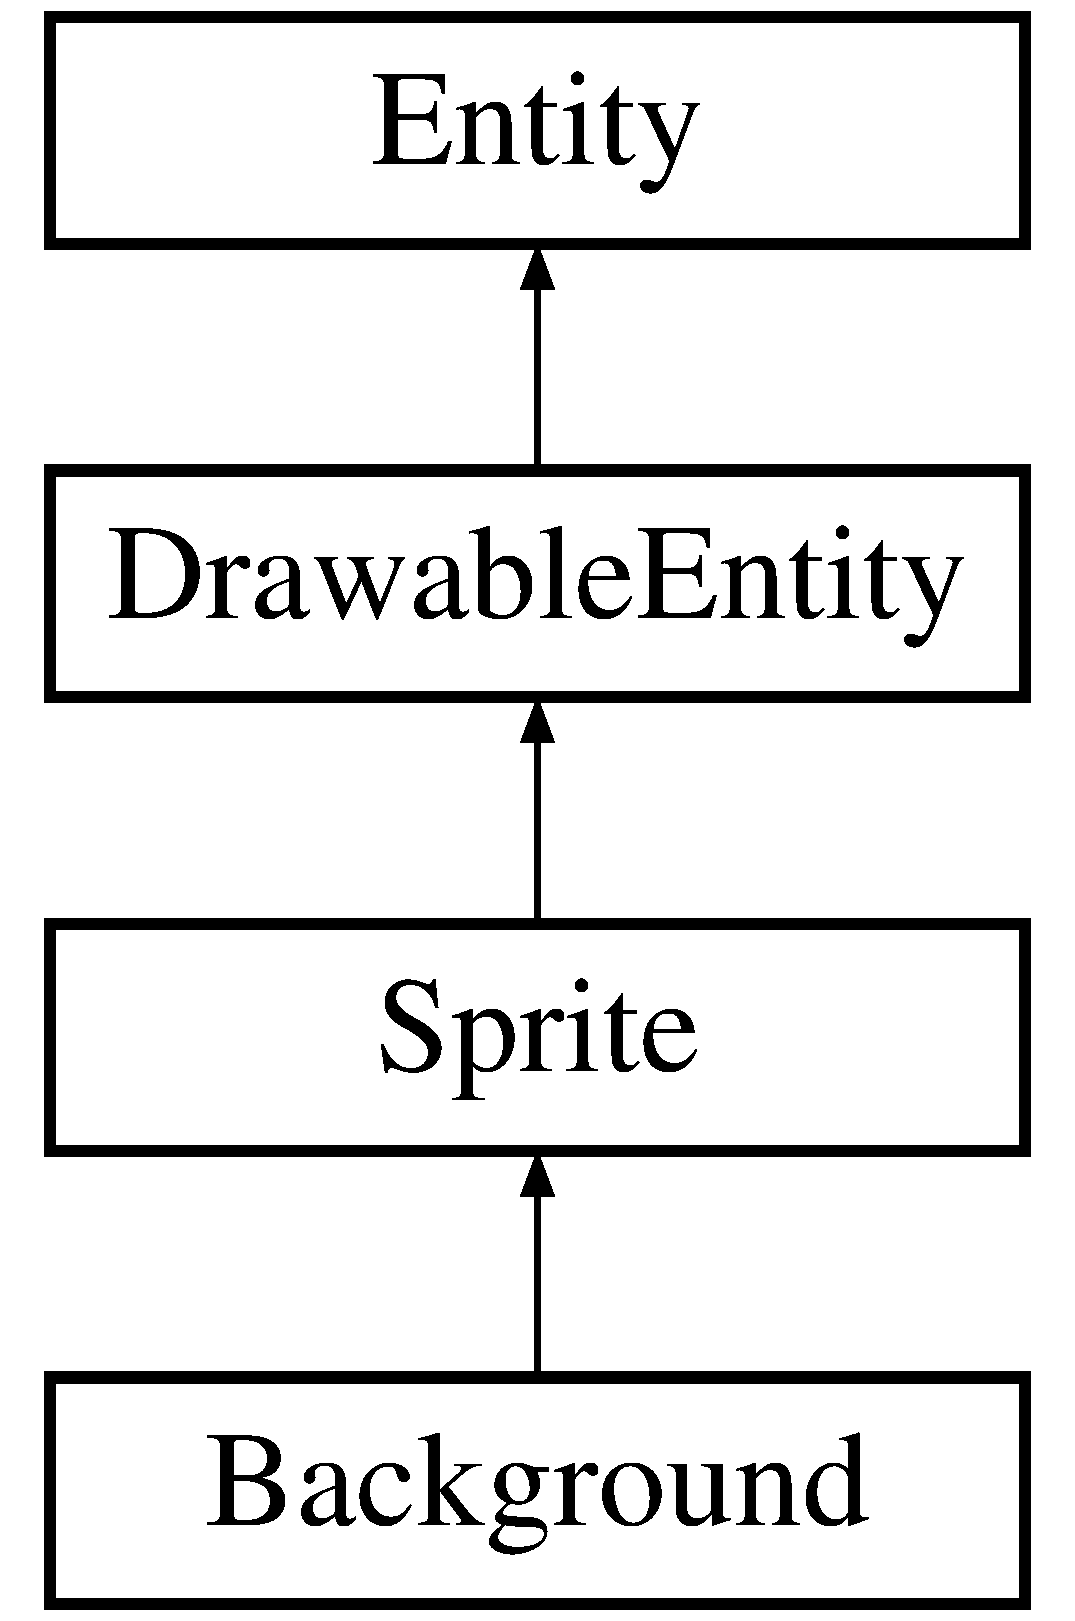
\includegraphics[height=4.000000cm]{class_background}
\end{center}
\end{figure}
\subsection*{Public Member Functions}
\begin{DoxyCompactItemize}
\item 
virtual \hyperlink{class_background_a8e03d13cc66a276ebd4ec1e6fc9e8c98}{$\sim$\+Background} ()
\begin{DoxyCompactList}\small\item\em Destroys the \hyperlink{class_background}{Background}. \end{DoxyCompactList}\item 
uint8\+\_\+t \hyperlink{class_background_ae4ae960cd876ef4a2f9fb6e0a7e8bc73}{init} (const std\+::string \&file\+\_\+path, const uint32\+\_\+t width, const uint32\+\_\+t height)
\begin{DoxyCompactList}\small\item\em Initializes the backgorund using a texture. \end{DoxyCompactList}\item 
void \hyperlink{class_background_af4a37c0ac474de5f65130cbef3d61379}{update} () override
\begin{DoxyCompactList}\small\item\em Updates the background position. \end{DoxyCompactList}\item 
void \hyperlink{class_background_a257183f6d077bbee005760813dbb0592}{draw} (sf\+::\+Render\+Window \&window) override
\begin{DoxyCompactList}\small\item\em Draws the graphic entity \hyperlink{class_background}{Background}. \end{DoxyCompactList}\item 
void \hyperlink{class_background_ad3559e8684aca155ae68d53374f3540d}{unuse} () override
\begin{DoxyCompactList}\small\item\em Resets the values of the background. \end{DoxyCompactList}\end{DoxyCompactItemize}
\subsection*{Static Public Member Functions}
\begin{DoxyCompactItemize}
\item 
static \hyperlink{class_background}{Background} $\ast$ \hyperlink{class_background_aafc5996195781b2d4bff7d170792425d}{Create\+Background} ()
\begin{DoxyCompactList}\small\item\em Factory that creates backgrounds. \end{DoxyCompactList}\end{DoxyCompactItemize}
\subsection*{Public Attributes}
\begin{DoxyCompactItemize}
\item 
\mbox{\Hypertarget{class_background_a9150d8924dc8e74ff9852d33cc0b574f}\label{class_background_a9150d8924dc8e74ff9852d33cc0b574f}} 
uint8\+\_\+t {\bfseries scrolls\+\_\+horizontally\+\_\+}
\item 
\mbox{\Hypertarget{class_background_aa26c61f1bbed1d8a8625b51bc3cc16dd}\label{class_background_aa26c61f1bbed1d8a8625b51bc3cc16dd}} 
uint8\+\_\+t {\bfseries scrolls\+\_\+vertically\+\_\+}
\item 
\mbox{\Hypertarget{class_background_a4402837678f3b72ac1f5803c97dfba28}\label{class_background_a4402837678f3b72ac1f5803c97dfba28}} 
sf\+::\+Vector2i {\bfseries speed\+\_\+}
\item 
\mbox{\Hypertarget{class_background_a515f93f6c513ec0519c02fa30c8bc5fa}\label{class_background_a515f93f6c513ec0519c02fa30c8bc5fa}} 
sf\+::\+Vector2i {\bfseries dimensions\+\_\+}
\item 
\mbox{\Hypertarget{class_background_abf90fe1fcc93375f86aee37a1dddbe37}\label{class_background_abf90fe1fcc93375f86aee37a1dddbe37}} 
sf\+::\+Vector2i {\bfseries background\+\_\+position\+\_\+}
\end{DoxyCompactItemize}
\subsection*{Additional Inherited Members}


\subsection{Detailed Description}
Graphic entity \hyperlink{class_background}{Background}. 

Class used to represent backgrounds. Used to stablish continuous movement to a sprite. 

\subsection{Constructor \& Destructor Documentation}
\mbox{\Hypertarget{class_background_a8e03d13cc66a276ebd4ec1e6fc9e8c98}\label{class_background_a8e03d13cc66a276ebd4ec1e6fc9e8c98}} 
\index{Background@{Background}!````~Background@{$\sim$\+Background}}
\index{````~Background@{$\sim$\+Background}!Background@{Background}}
\subsubsection{\texorpdfstring{$\sim$\+Background()}{~Background()}}
{\footnotesize\ttfamily virtual Background\+::$\sim$\+Background (\begin{DoxyParamCaption}{ }\end{DoxyParamCaption})\hspace{0.3cm}{\ttfamily [virtual]}}



Destroys the \hyperlink{class_background}{Background}. 

Destructor of the background

\begin{DoxyReturn}{Returns}
void 
\end{DoxyReturn}


\subsection{Member Function Documentation}
\mbox{\Hypertarget{class_background_aafc5996195781b2d4bff7d170792425d}\label{class_background_aafc5996195781b2d4bff7d170792425d}} 
\index{Background@{Background}!Create\+Background@{Create\+Background}}
\index{Create\+Background@{Create\+Background}!Background@{Background}}
\subsubsection{\texorpdfstring{Create\+Background()}{CreateBackground()}}
{\footnotesize\ttfamily static \hyperlink{class_background}{Background}$\ast$ Background\+::\+Create\+Background (\begin{DoxyParamCaption}{ }\end{DoxyParamCaption})\hspace{0.3cm}{\ttfamily [static]}}



Factory that creates backgrounds. 

Checks that the number of sprites didn\textquotesingle{}t pass the maxim amount established If you wish to create a \hyperlink{class_background}{Background} you must use this method. In case the maximum amount of sprites has been reached it will return nullptr. Otherwise it will return a pointer to a background. Note that it specifically uses the number of sprites as the background is by logic an sprite with movement.

\begin{DoxyReturn}{Returns}
Background$\ast$ returns the background created or nullptr if the maximum of sprites has been reached 
\end{DoxyReturn}
\mbox{\Hypertarget{class_background_a257183f6d077bbee005760813dbb0592}\label{class_background_a257183f6d077bbee005760813dbb0592}} 
\index{Background@{Background}!draw@{draw}}
\index{draw@{draw}!Background@{Background}}
\subsubsection{\texorpdfstring{draw()}{draw()}}
{\footnotesize\ttfamily void Background\+::draw (\begin{DoxyParamCaption}\item[{sf\+::\+Render\+Window \&}]{window }\end{DoxyParamCaption})\hspace{0.3cm}{\ttfamily [override]}, {\ttfamily [virtual]}}



Draws the graphic entity \hyperlink{class_background}{Background}. 

Draws the background using S\+F\+ML to the window passed by reference, note that the background doesn\textquotesingle{}t use the transformationso of it\textquotesingle{}s parent, you can set them bou they won\textquotesingle{}t have any effect over the background.

\begin{DoxyReturn}{Returns}
void 
\end{DoxyReturn}

\begin{DoxyParams}{Parameters}
{\em window} & S\+F\+ML Render\+Window passed by reference \\
\hline
\end{DoxyParams}


Reimplemented from \hyperlink{class_sprite_a067dfc27f53ce4d983db29407be1c11e}{Sprite}.

\mbox{\Hypertarget{class_background_ae4ae960cd876ef4a2f9fb6e0a7e8bc73}\label{class_background_ae4ae960cd876ef4a2f9fb6e0a7e8bc73}} 
\index{Background@{Background}!init@{init}}
\index{init@{init}!Background@{Background}}
\subsubsection{\texorpdfstring{init()}{init()}}
{\footnotesize\ttfamily uint8\+\_\+t Background\+::init (\begin{DoxyParamCaption}\item[{const std\+::string \&}]{file\+\_\+path,  }\item[{const uint32\+\_\+t}]{width,  }\item[{const uint32\+\_\+t}]{height }\end{DoxyParamCaption})}



Initializes the backgorund using a texture. 

Initializes the width height and path of a background

\begin{DoxyReturn}{Returns}
uint8\+\_\+t indicates if there was an error in the execution error-\/$>$1 ok-\/$>$0 
\end{DoxyReturn}

\begin{DoxyParams}{Parameters}
{\em width} & width the background will be initialized to \\
\hline
{\em height} & height the background will be initialized to \\
\hline
{\em file\+\_\+path} & image that will be used for the texture \\
\hline
\end{DoxyParams}
\mbox{\Hypertarget{class_background_ad3559e8684aca155ae68d53374f3540d}\label{class_background_ad3559e8684aca155ae68d53374f3540d}} 
\index{Background@{Background}!unuse@{unuse}}
\index{unuse@{unuse}!Background@{Background}}
\subsubsection{\texorpdfstring{unuse()}{unuse()}}
{\footnotesize\ttfamily void Background\+::unuse (\begin{DoxyParamCaption}{ }\end{DoxyParamCaption})\hspace{0.3cm}{\ttfamily [override]}, {\ttfamily [virtual]}}



Resets the values of the background. 

Sets the attributes of the background to a default value to return it to a pool and being able to reuse it later.

\begin{DoxyReturn}{Returns}
void 
\end{DoxyReturn}


Reimplemented from \hyperlink{class_sprite_a26066db75daec637f436d4635418059a}{Sprite}.

\mbox{\Hypertarget{class_background_af4a37c0ac474de5f65130cbef3d61379}\label{class_background_af4a37c0ac474de5f65130cbef3d61379}} 
\index{Background@{Background}!update@{update}}
\index{update@{update}!Background@{Background}}
\subsubsection{\texorpdfstring{update()}{update()}}
{\footnotesize\ttfamily void Background\+::update (\begin{DoxyParamCaption}{ }\end{DoxyParamCaption})\hspace{0.3cm}{\ttfamily [override]}, {\ttfamily [virtual]}}



Updates the background position. 

Updates the position of the background in the x,y axis if they are active, implementation of the update interface

\begin{DoxyReturn}{Returns}
void 
\end{DoxyReturn}


Reimplemented from \hyperlink{class_sprite_a1070fccd6830382b72e3f3a8785afc8c}{Sprite}.



The documentation for this class was generated from the following file\+:\begin{DoxyCompactItemize}
\item 
C\+:/\+E\+S\+A\+T/2pa\+\_\+ma\+\_\+martinezcajm/2d\+\_\+engine/include/background.\+h\end{DoxyCompactItemize}

\hypertarget{class_drawable_entity}{}\section{Drawable\+Entity Class Reference}
\label{class_drawable_entity}\index{Drawable\+Entity@{Drawable\+Entity}}


Drawable entity.  




{\ttfamily \#include $<$drawable\+\_\+entity.\+h$>$}

Inheritance diagram for Drawable\+Entity\+:\begin{figure}[H]
\begin{center}
\leavevmode
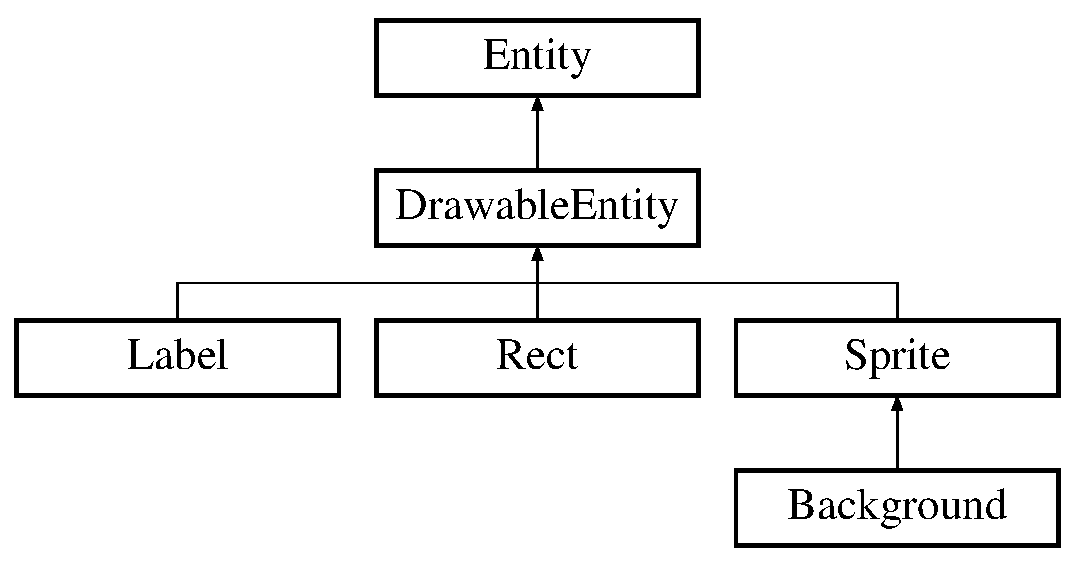
\includegraphics[height=3.555556cm]{class_drawable_entity}
\end{center}
\end{figure}
\subsection*{Public Member Functions}
\begin{DoxyCompactItemize}
\item 
\hyperlink{class_drawable_entity_a8e9f9afa7c76fdc19e27ca0975ffcb21}{Drawable\+Entity} ()
\begin{DoxyCompactList}\small\item\em Drawable entity constructor. \end{DoxyCompactList}\item 
virtual \hyperlink{class_drawable_entity_af688295ed4873a01b32862c3c0241933}{$\sim$\+Drawable\+Entity} ()
\begin{DoxyCompactList}\small\item\em Destroys the Drawable entity. \end{DoxyCompactList}\item 
void \hyperlink{class_drawable_entity_a3893879bf0710a7f5c5e7eb758ad7e96}{init} (const uint8\+\_\+t r, const uint8\+\_\+t g, const uint8\+\_\+t b, const uint8\+\_\+t a, const float px, const float py, const float rotation, const float scalex, const float scaley)
\begin{DoxyCompactList}\small\item\em Initializes the drawable entity. \end{DoxyCompactList}\item 
void \hyperlink{class_drawable_entity_a016d3d0cc80f9834918de44e0adb19fb}{move} (const float px, const float py)
\begin{DoxyCompactList}\small\item\em moves the entity \end{DoxyCompactList}\item 
virtual void \hyperlink{class_drawable_entity_a0b0db9c1325defed216d66a5b4cc755e}{draw} (sf\+::\+Render\+Window \&window)=0
\begin{DoxyCompactList}\small\item\em interface implementation of draw \end{DoxyCompactList}\item 
void \hyperlink{class_drawable_entity_a41ad5dfa5e9a5c366e05ba28bb469557}{draw\+With\+Transform} (sf\+::\+Render\+Window \&window, const sf\+::\+Drawable \&entity, const sf\+::\+Vector2f \&rotation\+\_\+origin)
\begin{DoxyCompactList}\small\item\em draws a drawable entity \end{DoxyCompactList}\item 
bool \hyperlink{class_drawable_entity_a4488d49a6e020b228aae6887ca6b644e}{check\+Collision} (const sf\+::\+Vector2f \&position)
\begin{DoxyCompactList}\small\item\em Checks if a point collides with the entity. \end{DoxyCompactList}\item 
bool \hyperlink{class_drawable_entity_a565c4767989b6390b06b52137b249ce5}{check\+Collision} (\hyperlink{class_drawable_entity}{Drawable\+Entity} \&entity)
\begin{DoxyCompactList}\small\item\em Checks if an entity collides with this entity. \end{DoxyCompactList}\item 
virtual sf\+::\+Float\+Rect \hyperlink{class_drawable_entity_a352a101e3be05d25e1a10e5f72ccb9e3}{get\+Boundaries} ()=0
\begin{DoxyCompactList}\small\item\em gets the boundaries of the drawable entity \end{DoxyCompactList}\item 
virtual void \hyperlink{class_drawable_entity_aabea8715834f6cee7fd36b038d1a4843}{unuse} () override
\begin{DoxyCompactList}\small\item\em Resets the values of the entity. \end{DoxyCompactList}\item 
virtual void \hyperlink{class_drawable_entity_acbf8317de062a2e0e79f646dbe75249c}{update} ()=0
\begin{DoxyCompactList}\small\item\em interface Update method \end{DoxyCompactList}\end{DoxyCompactItemize}
\subsection*{Public Attributes}
\begin{DoxyCompactItemize}
\item 
\mbox{\Hypertarget{class_drawable_entity_a7edd7e234484ae696a2820f186109929}\label{class_drawable_entity_a7edd7e234484ae696a2820f186109929}} 
int32\+\_\+t {\bfseries z\+\_\+order\+\_\+}
\item 
\mbox{\Hypertarget{class_drawable_entity_a883df88517413496ba69558f5f32623c}\label{class_drawable_entity_a883df88517413496ba69558f5f32623c}} 
float {\bfseries rotation\+\_\+}
\item 
\mbox{\Hypertarget{class_drawable_entity_abcda108a72f5c59464f65cbd8c405410}\label{class_drawable_entity_abcda108a72f5c59464f65cbd8c405410}} 
sf\+::\+Vector2f {\bfseries position\+\_\+}
\item 
\mbox{\Hypertarget{class_drawable_entity_a834104b0d2cddb9d03bffbf251547d90}\label{class_drawable_entity_a834104b0d2cddb9d03bffbf251547d90}} 
sf\+::\+Vector2f {\bfseries scale\+\_\+}
\item 
\mbox{\Hypertarget{class_drawable_entity_ad424f3d5b9ddbc6c556fbc64642e9153}\label{class_drawable_entity_ad424f3d5b9ddbc6c556fbc64642e9153}} 
sf\+::\+Color {\bfseries color\+\_\+}
\end{DoxyCompactItemize}
\subsection*{Additional Inherited Members}


\subsection{Detailed Description}
Drawable entity. 

Class used to specify the common methods and attributes of the entities that can be drawn. 

\subsection{Constructor \& Destructor Documentation}
\mbox{\Hypertarget{class_drawable_entity_a8e9f9afa7c76fdc19e27ca0975ffcb21}\label{class_drawable_entity_a8e9f9afa7c76fdc19e27ca0975ffcb21}} 
\index{Drawable\+Entity@{Drawable\+Entity}!Drawable\+Entity@{Drawable\+Entity}}
\index{Drawable\+Entity@{Drawable\+Entity}!Drawable\+Entity@{Drawable\+Entity}}
\subsubsection{\texorpdfstring{Drawable\+Entity()}{DrawableEntity()}}
{\footnotesize\ttfamily Drawable\+Entity\+::\+Drawable\+Entity (\begin{DoxyParamCaption}{ }\end{DoxyParamCaption})}



Drawable entity constructor. 

Drawable entity constructor

\begin{DoxyReturn}{Returns}
$\ast$\+Drawable\+Entity 
\end{DoxyReturn}
\mbox{\Hypertarget{class_drawable_entity_af688295ed4873a01b32862c3c0241933}\label{class_drawable_entity_af688295ed4873a01b32862c3c0241933}} 
\index{Drawable\+Entity@{Drawable\+Entity}!````~Drawable\+Entity@{$\sim$\+Drawable\+Entity}}
\index{````~Drawable\+Entity@{$\sim$\+Drawable\+Entity}!Drawable\+Entity@{Drawable\+Entity}}
\subsubsection{\texorpdfstring{$\sim$\+Drawable\+Entity()}{~DrawableEntity()}}
{\footnotesize\ttfamily virtual Drawable\+Entity\+::$\sim$\+Drawable\+Entity (\begin{DoxyParamCaption}{ }\end{DoxyParamCaption})\hspace{0.3cm}{\ttfamily [virtual]}}



Destroys the Drawable entity. 

Destructor of the drawable entity

\begin{DoxyReturn}{Returns}
void 
\end{DoxyReturn}


\subsection{Member Function Documentation}
\mbox{\Hypertarget{class_drawable_entity_a4488d49a6e020b228aae6887ca6b644e}\label{class_drawable_entity_a4488d49a6e020b228aae6887ca6b644e}} 
\index{Drawable\+Entity@{Drawable\+Entity}!check\+Collision@{check\+Collision}}
\index{check\+Collision@{check\+Collision}!Drawable\+Entity@{Drawable\+Entity}}
\subsubsection{\texorpdfstring{check\+Collision()}{checkCollision()}\hspace{0.1cm}{\footnotesize\ttfamily [1/2]}}
{\footnotesize\ttfamily bool Drawable\+Entity\+::check\+Collision (\begin{DoxyParamCaption}\item[{const sf\+::\+Vector2f \&}]{position }\end{DoxyParamCaption})}



Checks if a point collides with the entity. 

Checks if the point passed by reference collides with the boundaries.

\begin{DoxyReturn}{Returns}
bool returns true if the point collides and false if not. 
\end{DoxyReturn}

\begin{DoxyParams}{Parameters}
{\em sf\+::\+Vector2f} & point to check if collides with the entity \\
\hline
\end{DoxyParams}
\mbox{\Hypertarget{class_drawable_entity_a565c4767989b6390b06b52137b249ce5}\label{class_drawable_entity_a565c4767989b6390b06b52137b249ce5}} 
\index{Drawable\+Entity@{Drawable\+Entity}!check\+Collision@{check\+Collision}}
\index{check\+Collision@{check\+Collision}!Drawable\+Entity@{Drawable\+Entity}}
\subsubsection{\texorpdfstring{check\+Collision()}{checkCollision()}\hspace{0.1cm}{\footnotesize\ttfamily [2/2]}}
{\footnotesize\ttfamily bool Drawable\+Entity\+::check\+Collision (\begin{DoxyParamCaption}\item[{\hyperlink{class_drawable_entity}{Drawable\+Entity} \&}]{entity }\end{DoxyParamCaption})}



Checks if an entity collides with this entity. 

Checks if the entity passed by reference collides with the boundaries.

\begin{DoxyReturn}{Returns}
bool returns true if the point collides and false if not. 
\end{DoxyReturn}

\begin{DoxyParams}{Parameters}
{\em \hyperlink{class_drawable_entity}{Drawable\+Entity}} & entity to check if there\textquotesingle{}s a collision \\
\hline
\end{DoxyParams}
\mbox{\Hypertarget{class_drawable_entity_a0b0db9c1325defed216d66a5b4cc755e}\label{class_drawable_entity_a0b0db9c1325defed216d66a5b4cc755e}} 
\index{Drawable\+Entity@{Drawable\+Entity}!draw@{draw}}
\index{draw@{draw}!Drawable\+Entity@{Drawable\+Entity}}
\subsubsection{\texorpdfstring{draw()}{draw()}}
{\footnotesize\ttfamily virtual void Drawable\+Entity\+::draw (\begin{DoxyParamCaption}\item[{sf\+::\+Render\+Window \&}]{window }\end{DoxyParamCaption})\hspace{0.3cm}{\ttfamily [pure virtual]}}



interface implementation of draw 

Abstract implementation of the draw method for their children, needs the window were the entity will be drawn

\begin{DoxyReturn}{Returns}
void 
\end{DoxyReturn}

\begin{DoxyParams}{Parameters}
{\em window} & window in wich the entity will be drawn. \\
\hline
\end{DoxyParams}


Implemented in \hyperlink{class_sprite_a067dfc27f53ce4d983db29407be1c11e}{Sprite}, \hyperlink{class_rect_a57801edbfb2c000c631a610c59e7ff20}{Rect}, \hyperlink{class_background_a257183f6d077bbee005760813dbb0592}{Background}, and \hyperlink{class_label_aa0e2a948b68c7b70dde12b06b83a0cb1}{Label}.

\mbox{\Hypertarget{class_drawable_entity_a41ad5dfa5e9a5c366e05ba28bb469557}\label{class_drawable_entity_a41ad5dfa5e9a5c366e05ba28bb469557}} 
\index{Drawable\+Entity@{Drawable\+Entity}!draw\+With\+Transform@{draw\+With\+Transform}}
\index{draw\+With\+Transform@{draw\+With\+Transform}!Drawable\+Entity@{Drawable\+Entity}}
\subsubsection{\texorpdfstring{draw\+With\+Transform()}{drawWithTransform()}}
{\footnotesize\ttfamily void Drawable\+Entity\+::draw\+With\+Transform (\begin{DoxyParamCaption}\item[{sf\+::\+Render\+Window \&}]{window,  }\item[{const sf\+::\+Drawable \&}]{entity,  }\item[{const sf\+::\+Vector2f \&}]{rotation\+\_\+origin }\end{DoxyParamCaption})}



draws a drawable entity 

this method is in charge of applying the transformations that are common to all drawable\+\_\+entities using the transform class of S\+F\+ML (uses matrix) and finally drawing it to the window.

\begin{DoxyReturn}{Returns}
void 
\end{DoxyReturn}

\begin{DoxyParams}{Parameters}
{\em window} & window in wich the entity will be drawn. \\
\hline
{\em entity} & entity that will be drawn.  origin point from wich the rotation will be done. \\
\hline
\end{DoxyParams}
\mbox{\Hypertarget{class_drawable_entity_a352a101e3be05d25e1a10e5f72ccb9e3}\label{class_drawable_entity_a352a101e3be05d25e1a10e5f72ccb9e3}} 
\index{Drawable\+Entity@{Drawable\+Entity}!get\+Boundaries@{get\+Boundaries}}
\index{get\+Boundaries@{get\+Boundaries}!Drawable\+Entity@{Drawable\+Entity}}
\subsubsection{\texorpdfstring{get\+Boundaries()}{getBoundaries()}}
{\footnotesize\ttfamily virtual sf\+::\+Float\+Rect Drawable\+Entity\+::get\+Boundaries (\begin{DoxyParamCaption}{ }\end{DoxyParamCaption})\hspace{0.3cm}{\ttfamily [pure virtual]}}



gets the boundaries of the drawable entity 

Definition of the get\+Boundaries interface.

\begin{DoxyReturn}{Returns}
sf\+::\+Float\+Rect boundaries of the entity. 
\end{DoxyReturn}


Implemented in \hyperlink{class_sprite_add63c87af068cdcdb536eb1c82644ab4}{Sprite}, \hyperlink{class_label_a3eb456d7295b3d5af615b3dc6e761f4b}{Label}, and \hyperlink{class_rect_a17056b26af5522b024e9628386d34335}{Rect}.

\mbox{\Hypertarget{class_drawable_entity_a3893879bf0710a7f5c5e7eb758ad7e96}\label{class_drawable_entity_a3893879bf0710a7f5c5e7eb758ad7e96}} 
\index{Drawable\+Entity@{Drawable\+Entity}!init@{init}}
\index{init@{init}!Drawable\+Entity@{Drawable\+Entity}}
\subsubsection{\texorpdfstring{init()}{init()}}
{\footnotesize\ttfamily void Drawable\+Entity\+::init (\begin{DoxyParamCaption}\item[{const uint8\+\_\+t}]{r,  }\item[{const uint8\+\_\+t}]{g,  }\item[{const uint8\+\_\+t}]{b,  }\item[{const uint8\+\_\+t}]{a,  }\item[{const float}]{px,  }\item[{const float}]{py,  }\item[{const float}]{rotation,  }\item[{const float}]{scalex,  }\item[{const float}]{scaley }\end{DoxyParamCaption})}



Initializes the drawable entity. 

Initializes the drawable entity

\begin{DoxyReturn}{Returns}
void 
\end{DoxyReturn}

\begin{DoxyParams}{Parameters}
{\em r} & color red component of the label we want to create \\
\hline
{\em g} & color blue component of the label we want to create \\
\hline
{\em b} & color green component of the label we want to create \\
\hline
{\em a} & alpha channel of the color of the label we want to create \\
\hline
{\em px} & x position in the window \\
\hline
{\em py} & y position in the window \\
\hline
{\em rotation} & rotation in degrees \\
\hline
{\em scalex} & scale quantity at x axis \\
\hline
{\em scaley} & scale quantity at y axis \\
\hline
\end{DoxyParams}
\mbox{\Hypertarget{class_drawable_entity_a016d3d0cc80f9834918de44e0adb19fb}\label{class_drawable_entity_a016d3d0cc80f9834918de44e0adb19fb}} 
\index{Drawable\+Entity@{Drawable\+Entity}!move@{move}}
\index{move@{move}!Drawable\+Entity@{Drawable\+Entity}}
\subsubsection{\texorpdfstring{move()}{move()}}
{\footnotesize\ttfamily void Drawable\+Entity\+::move (\begin{DoxyParamCaption}\item[{const float}]{px,  }\item[{const float}]{py }\end{DoxyParamCaption})}



moves the entity 

moves the entity a number of points from it\textquotesingle{}s original position x, y

\begin{DoxyReturn}{Returns}
void 
\end{DoxyReturn}

\begin{DoxyParams}{Parameters}
{\em px} & quantity the entity will move in the x axis \\
\hline
{\em py} & quantity the entity will move in the y axis \\
\hline
\end{DoxyParams}
\mbox{\Hypertarget{class_drawable_entity_aabea8715834f6cee7fd36b038d1a4843}\label{class_drawable_entity_aabea8715834f6cee7fd36b038d1a4843}} 
\index{Drawable\+Entity@{Drawable\+Entity}!unuse@{unuse}}
\index{unuse@{unuse}!Drawable\+Entity@{Drawable\+Entity}}
\subsubsection{\texorpdfstring{unuse()}{unuse()}}
{\footnotesize\ttfamily virtual void Drawable\+Entity\+::unuse (\begin{DoxyParamCaption}{ }\end{DoxyParamCaption})\hspace{0.3cm}{\ttfamily [override]}, {\ttfamily [virtual]}}



Resets the values of the entity. 

Sets the attributes of the object to return it to a pool and being able to reuse it later.

\begin{DoxyReturn}{Returns}
void 
\end{DoxyReturn}


Reimplemented from \hyperlink{class_entity_a7b87e24b0d790b2c182fad8aa572455c}{Entity}.



Reimplemented in \hyperlink{class_sprite_a26066db75daec637f436d4635418059a}{Sprite}, \hyperlink{class_label_aa6a355fe8daa25c3739affcf66d66f7f}{Label}, \hyperlink{class_rect_a85afbe7fde3b74bd81c07cc58d5c61bd}{Rect}, and \hyperlink{class_background_ad3559e8684aca155ae68d53374f3540d}{Background}.

\mbox{\Hypertarget{class_drawable_entity_acbf8317de062a2e0e79f646dbe75249c}\label{class_drawable_entity_acbf8317de062a2e0e79f646dbe75249c}} 
\index{Drawable\+Entity@{Drawable\+Entity}!update@{update}}
\index{update@{update}!Drawable\+Entity@{Drawable\+Entity}}
\subsubsection{\texorpdfstring{update()}{update()}}
{\footnotesize\ttfamily virtual void Drawable\+Entity\+::update (\begin{DoxyParamCaption}{ }\end{DoxyParamCaption})\hspace{0.3cm}{\ttfamily [pure virtual]}}



interface Update method 

Definition of the update interface for the drawable entities

\begin{DoxyReturn}{Returns}
void 
\end{DoxyReturn}


Implemented in \hyperlink{class_sprite_a1070fccd6830382b72e3f3a8785afc8c}{Sprite}, \hyperlink{class_player_abe7d0a24ffd93ba0bc4eea860b10eb09}{Player}, \hyperlink{class_ball_a26c877660343d086a9d45891659474f8}{Ball}, \hyperlink{class_label_adcd154f9e53d277c1b7a11bd058936a0}{Label}, \hyperlink{class_rect_af74b7ea3228d0d7b4c40bb8fe6daed63}{Rect}, \hyperlink{class_brick_a4debb742abe5d19442d910bb8ecf083e}{Brick}, and \hyperlink{class_background_af4a37c0ac474de5f65130cbef3d61379}{Background}.



The documentation for this class was generated from the following file\+:\begin{DoxyCompactItemize}
\item 
C\+:/\+E\+S\+A\+T/2pa\+\_\+ma\+\_\+martinezcajm/2d\+\_\+engine/include/drawable\+\_\+entity.\+h\end{DoxyCompactItemize}

\hypertarget{class_entity}{}\section{Entity Class Reference}
\label{class_entity}\index{Entity@{Entity}}


entity  




{\ttfamily \#include $<$entity.\+h$>$}

Inheritance diagram for Entity\+:\begin{figure}[H]
\begin{center}
\leavevmode
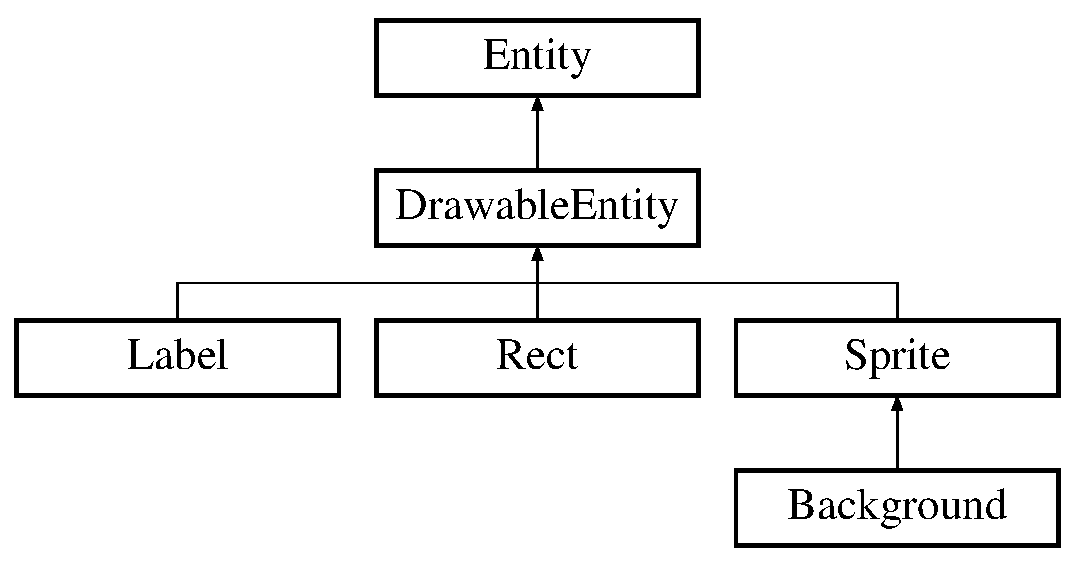
\includegraphics[height=3.555556cm]{class_entity}
\end{center}
\end{figure}
\subsection*{Public Types}
\begin{DoxyCompactItemize}
\item 
\mbox{\Hypertarget{class_entity_a0e96d5b4903c3e32e07780aa12fe075b}\label{class_entity_a0e96d5b4903c3e32e07780aa12fe075b}} 
enum {\bfseries Type} \{ \newline
{\bfseries k\+Rect} = 0, 
{\bfseries k\+Background} = 1, 
{\bfseries k\+Label} = 2, 
{\bfseries k\+Sprite} = 3, 
\newline
{\bfseries k\+Wall} = 4, 
{\bfseries k\+Brick} = 5, 
{\bfseries k\+Ball} = 6, 
{\bfseries k\+Player} = 7
 \}
\end{DoxyCompactItemize}
\subsection*{Public Member Functions}
\begin{DoxyCompactItemize}
\item 
\hyperlink{class_entity_a980f368aa07ce358583982821533a54a}{Entity} ()
\begin{DoxyCompactList}\small\item\em \hyperlink{class_entity}{Entity} constructor. \end{DoxyCompactList}\item 
virtual \hyperlink{class_entity_a6216319e71da21b7708bbfeb537c4d0f}{$\sim$\+Entity} ()=0
\begin{DoxyCompactList}\small\item\em Destroys the \hyperlink{class_entity}{Entity}. \end{DoxyCompactList}\item 
\hyperlink{class_entity_ad758dc48d715e48ada4193517f1d32ea}{Entity} (const \hyperlink{class_entity}{Entity} \&o)
\begin{DoxyCompactList}\small\item\em \hyperlink{class_entity}{Entity} copy constructor. \end{DoxyCompactList}\item 
void \hyperlink{class_entity_a085fa2dd2c2b1f3f60d601a68d5c6773}{init} (const uint32\+\_\+t tag)
\begin{DoxyCompactList}\small\item\em Initializes the \hyperlink{class_entity}{Entity}. \end{DoxyCompactList}\item 
void \hyperlink{class_entity_a93bfb0b92c06297c207fad4164810fed}{init} ()
\begin{DoxyCompactList}\small\item\em Initializes the \hyperlink{class_entity}{Entity}. \end{DoxyCompactList}\item 
uint32\+\_\+t \hyperlink{class_entity_ae4a75e659a4426f57f5c1d44f1b8ef34}{id} ()
\begin{DoxyCompactList}\small\item\em Getter of the id. \end{DoxyCompactList}\item 
virtual void \hyperlink{class_entity_a7b87e24b0d790b2c182fad8aa572455c}{unuse} ()
\begin{DoxyCompactList}\small\item\em Resets the values of the entity. \end{DoxyCompactList}\item 
Type \hyperlink{class_entity_a57c1ccf94325b1b771f4656178ab2b81}{type} ()
\begin{DoxyCompactList}\small\item\em Getter of the type. \end{DoxyCompactList}\end{DoxyCompactItemize}
\subsection*{Public Attributes}
\begin{DoxyCompactItemize}
\item 
\mbox{\Hypertarget{class_entity_aa9f75ea7b1041547a1b610a9b2f064c0}\label{class_entity_aa9f75ea7b1041547a1b610a9b2f064c0}} 
int {\bfseries tag\+\_\+}
\item 
\mbox{\Hypertarget{class_entity_a6f99bc47ee1c35ac95a36a5facd15e5d}\label{class_entity_a6f99bc47ee1c35ac95a36a5facd15e5d}} 
uint8\+\_\+t {\bfseries selection\+\_\+tag\+\_\+}
\item 
\mbox{\Hypertarget{class_entity_a7816e789062febe058b98ce695539c59}\label{class_entity_a7816e789062febe058b98ce695539c59}} 
uint8\+\_\+t {\bfseries active\+\_\+}
\end{DoxyCompactItemize}
\subsection*{Protected Attributes}
\begin{DoxyCompactItemize}
\item 
\mbox{\Hypertarget{class_entity_a4fa6e00c39af69477dc64c27e29ab77e}\label{class_entity_a4fa6e00c39af69477dc64c27e29ab77e}} 
Type {\bfseries type\+\_\+}
\end{DoxyCompactItemize}


\subsection{Detailed Description}
entity 

Atomic class of the elements of our engine. 

\subsection{Constructor \& Destructor Documentation}
\mbox{\Hypertarget{class_entity_a980f368aa07ce358583982821533a54a}\label{class_entity_a980f368aa07ce358583982821533a54a}} 
\index{Entity@{Entity}!Entity@{Entity}}
\index{Entity@{Entity}!Entity@{Entity}}
\subsubsection{\texorpdfstring{Entity()}{Entity()}\hspace{0.1cm}{\footnotesize\ttfamily [1/2]}}
{\footnotesize\ttfamily Entity\+::\+Entity (\begin{DoxyParamCaption}{ }\end{DoxyParamCaption})}



\hyperlink{class_entity}{Entity} constructor. 

Base constructor of entity

\begin{DoxyReturn}{Returns}
$\ast$\+Entity 
\end{DoxyReturn}
\mbox{\Hypertarget{class_entity_a6216319e71da21b7708bbfeb537c4d0f}\label{class_entity_a6216319e71da21b7708bbfeb537c4d0f}} 
\index{Entity@{Entity}!````~Entity@{$\sim$\+Entity}}
\index{````~Entity@{$\sim$\+Entity}!Entity@{Entity}}
\subsubsection{\texorpdfstring{$\sim$\+Entity()}{~Entity()}}
{\footnotesize\ttfamily virtual Entity\+::$\sim$\+Entity (\begin{DoxyParamCaption}{ }\end{DoxyParamCaption})\hspace{0.3cm}{\ttfamily [inline]}, {\ttfamily [pure virtual]}}



Destroys the \hyperlink{class_entity}{Entity}. 

Destructor of the entity

\begin{DoxyReturn}{Returns}
void 
\end{DoxyReturn}
\mbox{\Hypertarget{class_entity_ad758dc48d715e48ada4193517f1d32ea}\label{class_entity_ad758dc48d715e48ada4193517f1d32ea}} 
\index{Entity@{Entity}!Entity@{Entity}}
\index{Entity@{Entity}!Entity@{Entity}}
\subsubsection{\texorpdfstring{Entity()}{Entity()}\hspace{0.1cm}{\footnotesize\ttfamily [2/2]}}
{\footnotesize\ttfamily Entity\+::\+Entity (\begin{DoxyParamCaption}\item[{const \hyperlink{class_entity}{Entity} \&}]{o }\end{DoxyParamCaption})}



\hyperlink{class_entity}{Entity} copy constructor. 

Personal \hyperlink{class_entity}{Entity} copy constructor taking into account the id.

\begin{DoxyReturn}{Returns}
$\ast$\+Entity 
\end{DoxyReturn}


\subsection{Member Function Documentation}
\mbox{\Hypertarget{class_entity_ae4a75e659a4426f57f5c1d44f1b8ef34}\label{class_entity_ae4a75e659a4426f57f5c1d44f1b8ef34}} 
\index{Entity@{Entity}!id@{id}}
\index{id@{id}!Entity@{Entity}}
\subsubsection{\texorpdfstring{id()}{id()}}
{\footnotesize\ttfamily uint32\+\_\+t Entity\+::id (\begin{DoxyParamCaption}{ }\end{DoxyParamCaption})}



Getter of the id. 

Returns the value of the id

\begin{DoxyReturn}{Returns}
uint32\+\_\+t id of the entity 
\end{DoxyReturn}
\mbox{\Hypertarget{class_entity_a085fa2dd2c2b1f3f60d601a68d5c6773}\label{class_entity_a085fa2dd2c2b1f3f60d601a68d5c6773}} 
\index{Entity@{Entity}!init@{init}}
\index{init@{init}!Entity@{Entity}}
\subsubsection{\texorpdfstring{init()}{init()}\hspace{0.1cm}{\footnotesize\ttfamily [1/2]}}
{\footnotesize\ttfamily void Entity\+::init (\begin{DoxyParamCaption}\item[{const uint32\+\_\+t}]{tag }\end{DoxyParamCaption})}



Initializes the \hyperlink{class_entity}{Entity}. 

Initializes an entity with a tag

\begin{DoxyReturn}{Returns}
void 
\end{DoxyReturn}

\begin{DoxyParams}{Parameters}
{\em tag} & unsigned int used to group entities \\
\hline
\end{DoxyParams}
\mbox{\Hypertarget{class_entity_a93bfb0b92c06297c207fad4164810fed}\label{class_entity_a93bfb0b92c06297c207fad4164810fed}} 
\index{Entity@{Entity}!init@{init}}
\index{init@{init}!Entity@{Entity}}
\subsubsection{\texorpdfstring{init()}{init()}\hspace{0.1cm}{\footnotesize\ttfamily [2/2]}}
{\footnotesize\ttfamily void Entity\+::init (\begin{DoxyParamCaption}{ }\end{DoxyParamCaption})}



Initializes the \hyperlink{class_entity}{Entity}. 

Initializes an entity with default values

\begin{DoxyReturn}{Returns}
void 
\end{DoxyReturn}

\begin{DoxyParams}{Parameters}
{\em tag} & unsigned int used to group entities \\
\hline
\end{DoxyParams}
\mbox{\Hypertarget{class_entity_a57c1ccf94325b1b771f4656178ab2b81}\label{class_entity_a57c1ccf94325b1b771f4656178ab2b81}} 
\index{Entity@{Entity}!type@{type}}
\index{type@{type}!Entity@{Entity}}
\subsubsection{\texorpdfstring{type()}{type()}}
{\footnotesize\ttfamily Type Entity\+::type (\begin{DoxyParamCaption}{ }\end{DoxyParamCaption})}



Getter of the type. 

Returns the type of the entity

\begin{DoxyReturn}{Returns}
Type type of the entity 
\end{DoxyReturn}
\mbox{\Hypertarget{class_entity_a7b87e24b0d790b2c182fad8aa572455c}\label{class_entity_a7b87e24b0d790b2c182fad8aa572455c}} 
\index{Entity@{Entity}!unuse@{unuse}}
\index{unuse@{unuse}!Entity@{Entity}}
\subsubsection{\texorpdfstring{unuse()}{unuse()}}
{\footnotesize\ttfamily virtual void Entity\+::unuse (\begin{DoxyParamCaption}{ }\end{DoxyParamCaption})\hspace{0.3cm}{\ttfamily [virtual]}}



Resets the values of the entity. 

Sets the attributes of the object to return it to a pool and being able to reuse it later.

\begin{DoxyReturn}{Returns}
void 
\end{DoxyReturn}


Reimplemented in \hyperlink{class_drawable_entity_aabea8715834f6cee7fd36b038d1a4843}{Drawable\+Entity}, \hyperlink{class_sprite_a26066db75daec637f436d4635418059a}{Sprite}, \hyperlink{class_label_aa6a355fe8daa25c3739affcf66d66f7f}{Label}, \hyperlink{class_rect_a85afbe7fde3b74bd81c07cc58d5c61bd}{Rect}, and \hyperlink{class_background_ad3559e8684aca155ae68d53374f3540d}{Background}.



The documentation for this class was generated from the following file\+:\begin{DoxyCompactItemize}
\item 
C\+:/\+E\+S\+A\+T/2pa\+\_\+ma\+\_\+martinezcajm/2d\+\_\+engine/include/entity.\+h\end{DoxyCompactItemize}

\hypertarget{class_game}{}\section{Game Class Reference}
\label{class_game}\index{Game@{Game}}


{\ttfamily \#include $<$game.\+h$>$}

\subsection*{Public Member Functions}
\begin{DoxyCompactItemize}
\item 
\hyperlink{class_game_ad59df6562a58a614fda24622d3715b65}{Game} ()
\item 
\hyperlink{class_game_ae3d112ca6e0e55150d2fdbc704474530}{$\sim$\+Game} ()
\item 
void \hyperlink{class_game_a6f3a33940524b6ba9d83f627ccb14bbf}{init} ()
\item 
void \hyperlink{class_game_a815a3ec2787b4b1c4077d28165c380e8}{process\+Input} ()
\item 
void \hyperlink{class_game_a67a8c5c0356c9ad33fac1abc435a3746}{update\+Game} ()
\item 
void \hyperlink{class_game_a4573580347746dbb7dbe568383682ed3}{render\+Game} ()
\item 
void \hyperlink{class_game_a81abd2f677aba0c3f068c902d690e2fb}{update\+Editor} ()
\item 
void \hyperlink{class_game_a204ea65111892ca826f3a65cc8818ea7}{render\+Editor} ()
\item 
void \hyperlink{class_game_ae89e277761b7dc5bc7a23fd1b4c6f17d}{main\+Loop} ()
\item 
void \hyperlink{class_game_a4a803542276ea0497ad3a87b8983dd67}{finish} ()
\item 
void \hyperlink{class_game_a828811993f0d93a72758b05c98609540}{render\+UI} ()
\item 
void \hyperlink{class_game_a0a41188d1bfa82e9e0cdda1c0530a389}{Ui\+Load\+Common\+Values\+Edit} (\hyperlink{class_drawable_entity}{Drawable\+Entity} \&d\+\_\+entity)
\item 
void \hyperlink{class_game_a8710233ba10c51897d95b176f1bac5ca}{Ui\+Load\+Rect\+Values\+Edit} (\hyperlink{class_rect}{Rect} \&rect)
\item 
void \hyperlink{class_game_a895e8ae5390fcd21a903623a23ceeaac}{Ui\+Load\+Label\+Values\+Edit} (\hyperlink{class_label}{Label} \&label)
\item 
void \hyperlink{class_game_a65b1b506f6c9ffb4006e94680e05cd04}{Ui\+Load\+Background\+Values\+Edit} (\hyperlink{class_background}{Background} \&bg)
\item 
void \hyperlink{class_game_a184082948455436281839a2e96279e17}{Ui\+Load\+Menu} ()
\item 
void \hyperlink{class_game_aa18ae3db4c6d5b2fac2080afcd8e6790}{Ui\+Start\+Game\+Menu} ()
\end{DoxyCompactItemize}
\subsection*{Public Attributes}
\begin{DoxyCompactItemize}
\item 
\mbox{\Hypertarget{class_game_abdaa5299f22a22a628149cda5040c5c8}\label{class_game_abdaa5299f22a22a628149cda5040c5c8}} 
\hyperlink{class_game_manager}{Game\+Manager} \& {\bfseries GM} = \hyperlink{class_game_manager_afa37ab23c040b5225d567d4c9ab854e1}{Game\+Manager\+::instance}()
\item 
\mbox{\Hypertarget{class_game_aa22c10008978460e1dea4d6fbfa70b53}\label{class_game_aa22c10008978460e1dea4d6fbfa70b53}} 
\hyperlink{class_pool}{Pool} \& {\bfseries P\+O\+OL} = \hyperlink{class_pool_a20e44e0054d4eedf57f1943b87c06e20}{Pool\+::instance}()
\item 
\mbox{\Hypertarget{class_game_af4325db0c4cd8e4f51fd2b3567191d66}\label{class_game_af4325db0c4cd8e4f51fd2b3567191d66}} 
bool {\bfseries game\+\_\+over\+\_\+}
\item 
\mbox{\Hypertarget{class_game_acd6e7363beb1cdf8a208f07ec41f39ae}\label{class_game_acd6e7363beb1cdf8a208f07ec41f39ae}} 
char const  $\ast$ {\bfseries k\+Filter\+Patterns\+Json} \mbox{[}1\mbox{]} = \{ \char`\"{}$\ast$.json\char`\"{} \}
\item 
\mbox{\Hypertarget{class_game_a6abb1fb644b47a9ad92cad622b1b7222}\label{class_game_a6abb1fb644b47a9ad92cad622b1b7222}} 
char const  $\ast$ {\bfseries k\+Filter\+Patterns\+Image} \mbox{[}3\mbox{]} = \{ \char`\"{}$\ast$.png\char`\"{},\char`\"{}$\ast$.jpeg\char`\"{}, \char`\"{}$\ast$.jpg\char`\"{} \}
\end{DoxyCompactItemize}


\subsection{Detailed Description}
Main class of the editor

This class contains the main bucle of the game and editor 

\subsection{Constructor \& Destructor Documentation}
\mbox{\Hypertarget{class_game_ad59df6562a58a614fda24622d3715b65}\label{class_game_ad59df6562a58a614fda24622d3715b65}} 
\index{Game@{Game}!Game@{Game}}
\index{Game@{Game}!Game@{Game}}
\subsubsection{\texorpdfstring{Game()}{Game()}}
{\footnotesize\ttfamily Game\+::\+Game (\begin{DoxyParamCaption}{ }\end{DoxyParamCaption})}

the game

Constructor of the game

\begin{DoxyReturn}{Returns}
void 
\end{DoxyReturn}
\mbox{\Hypertarget{class_game_ae3d112ca6e0e55150d2fdbc704474530}\label{class_game_ae3d112ca6e0e55150d2fdbc704474530}} 
\index{Game@{Game}!````~Game@{$\sim$\+Game}}
\index{````~Game@{$\sim$\+Game}!Game@{Game}}
\subsubsection{\texorpdfstring{$\sim$\+Game()}{~Game()}}
{\footnotesize\ttfamily Game\+::$\sim$\+Game (\begin{DoxyParamCaption}{ }\end{DoxyParamCaption})}

the game

Destructor of the game

\begin{DoxyReturn}{Returns}
void 
\end{DoxyReturn}


\subsection{Member Function Documentation}
\mbox{\Hypertarget{class_game_a4a803542276ea0497ad3a87b8983dd67}\label{class_game_a4a803542276ea0497ad3a87b8983dd67}} 
\index{Game@{Game}!finish@{finish}}
\index{finish@{finish}!Game@{Game}}
\subsubsection{\texorpdfstring{finish()}{finish()}}
{\footnotesize\ttfamily void Game\+::finish (\begin{DoxyParamCaption}{ }\end{DoxyParamCaption})}

the game

Free the memoryof the elements of the game

\begin{DoxyReturn}{Returns}
void 
\end{DoxyReturn}
\mbox{\Hypertarget{class_game_a6f3a33940524b6ba9d83f627ccb14bbf}\label{class_game_a6f3a33940524b6ba9d83f627ccb14bbf}} 
\index{Game@{Game}!init@{init}}
\index{init@{init}!Game@{Game}}
\subsubsection{\texorpdfstring{init()}{init()}}
{\footnotesize\ttfamily void Game\+::init (\begin{DoxyParamCaption}{ }\end{DoxyParamCaption})}

the game

Initializes the necesary objects for the game.

\begin{DoxyReturn}{Returns}
void 
\end{DoxyReturn}
\mbox{\Hypertarget{class_game_ae89e277761b7dc5bc7a23fd1b4c6f17d}\label{class_game_ae89e277761b7dc5bc7a23fd1b4c6f17d}} 
\index{Game@{Game}!main\+Loop@{main\+Loop}}
\index{main\+Loop@{main\+Loop}!Game@{Game}}
\subsubsection{\texorpdfstring{main\+Loop()}{mainLoop()}}
{\footnotesize\ttfamily void Game\+::main\+Loop (\begin{DoxyParamCaption}{ }\end{DoxyParamCaption})}

the game loop

Process the game loop.

\begin{DoxyReturn}{Returns}
void 
\end{DoxyReturn}
\mbox{\Hypertarget{class_game_a815a3ec2787b4b1c4077d28165c380e8}\label{class_game_a815a3ec2787b4b1c4077d28165c380e8}} 
\index{Game@{Game}!process\+Input@{process\+Input}}
\index{process\+Input@{process\+Input}!Game@{Game}}
\subsubsection{\texorpdfstring{process\+Input()}{processInput()}}
{\footnotesize\ttfamily void Game\+::process\+Input (\begin{DoxyParamCaption}{ }\end{DoxyParamCaption})}

the inputs

Check the inputs and change the game stats for do the uptade.

\begin{DoxyReturn}{Returns}
void 
\end{DoxyReturn}
\mbox{\Hypertarget{class_game_a204ea65111892ca826f3a65cc8818ea7}\label{class_game_a204ea65111892ca826f3a65cc8818ea7}} 
\index{Game@{Game}!render\+Editor@{render\+Editor}}
\index{render\+Editor@{render\+Editor}!Game@{Game}}
\subsubsection{\texorpdfstring{render\+Editor()}{renderEditor()}}
{\footnotesize\ttfamily void Game\+::render\+Editor (\begin{DoxyParamCaption}{ }\end{DoxyParamCaption})}

the game entities

Draw all the entities of the game and the UI of the editor

\begin{DoxyReturn}{Returns}
void 
\end{DoxyReturn}
\mbox{\Hypertarget{class_game_a4573580347746dbb7dbe568383682ed3}\label{class_game_a4573580347746dbb7dbe568383682ed3}} 
\index{Game@{Game}!render\+Game@{render\+Game}}
\index{render\+Game@{render\+Game}!Game@{Game}}
\subsubsection{\texorpdfstring{render\+Game()}{renderGame()}}
{\footnotesize\ttfamily void Game\+::render\+Game (\begin{DoxyParamCaption}{ }\end{DoxyParamCaption})}

the game entities

Draw all the entities of the game

\begin{DoxyReturn}{Returns}
void 
\end{DoxyReturn}
\mbox{\Hypertarget{class_game_a828811993f0d93a72758b05c98609540}\label{class_game_a828811993f0d93a72758b05c98609540}} 
\index{Game@{Game}!render\+UI@{render\+UI}}
\index{render\+UI@{render\+UI}!Game@{Game}}
\subsubsection{\texorpdfstring{render\+U\+I()}{renderUI()}}
{\footnotesize\ttfamily void Game\+::render\+UI (\begin{DoxyParamCaption}{ }\end{DoxyParamCaption})}

the UI

Function in charge of rendering the UI

\begin{DoxyReturn}{Returns}
void 
\end{DoxyReturn}
\mbox{\Hypertarget{class_game_a65b1b506f6c9ffb4006e94680e05cd04}\label{class_game_a65b1b506f6c9ffb4006e94680e05cd04}} 
\index{Game@{Game}!Ui\+Load\+Background\+Values\+Edit@{Ui\+Load\+Background\+Values\+Edit}}
\index{Ui\+Load\+Background\+Values\+Edit@{Ui\+Load\+Background\+Values\+Edit}!Game@{Game}}
\subsubsection{\texorpdfstring{Ui\+Load\+Background\+Values\+Edit()}{UiLoadBackgroundValuesEdit()}}
{\footnotesize\ttfamily void Game\+::\+Ui\+Load\+Background\+Values\+Edit (\begin{DoxyParamCaption}\item[{\hyperlink{class_background}{Background} \&}]{bg }\end{DoxyParamCaption})}

the edit values of \hyperlink{class_background}{Background} entity

Loads the edit values of \hyperlink{class_background}{Background} entity\+: speed, vertical movememnt, horizaontal\+\_\+movement...

\begin{DoxyReturn}{Returns}
void 
\end{DoxyReturn}

\begin{DoxyParams}{Parameters}
{\em reference} & to the background whose values will be loaded at the UI \\
\hline
\end{DoxyParams}
\mbox{\Hypertarget{class_game_a0a41188d1bfa82e9e0cdda1c0530a389}\label{class_game_a0a41188d1bfa82e9e0cdda1c0530a389}} 
\index{Game@{Game}!Ui\+Load\+Common\+Values\+Edit@{Ui\+Load\+Common\+Values\+Edit}}
\index{Ui\+Load\+Common\+Values\+Edit@{Ui\+Load\+Common\+Values\+Edit}!Game@{Game}}
\subsubsection{\texorpdfstring{Ui\+Load\+Common\+Values\+Edit()}{UiLoadCommonValuesEdit()}}
{\footnotesize\ttfamily void Game\+::\+Ui\+Load\+Common\+Values\+Edit (\begin{DoxyParamCaption}\item[{\hyperlink{class_drawable_entity}{Drawable\+Entity} \&}]{d\+\_\+entity }\end{DoxyParamCaption})}

the edit values of Drawable entity

Loads the edit values of Drawable entity\+: transformations, color, position...

\begin{DoxyReturn}{Returns}
void 
\end{DoxyReturn}

\begin{DoxyParams}{Parameters}
{\em reference} & to the drawable entity whose values will be loaded at the UI \\
\hline
\end{DoxyParams}
\mbox{\Hypertarget{class_game_a895e8ae5390fcd21a903623a23ceeaac}\label{class_game_a895e8ae5390fcd21a903623a23ceeaac}} 
\index{Game@{Game}!Ui\+Load\+Label\+Values\+Edit@{Ui\+Load\+Label\+Values\+Edit}}
\index{Ui\+Load\+Label\+Values\+Edit@{Ui\+Load\+Label\+Values\+Edit}!Game@{Game}}
\subsubsection{\texorpdfstring{Ui\+Load\+Label\+Values\+Edit()}{UiLoadLabelValuesEdit()}}
{\footnotesize\ttfamily void Game\+::\+Ui\+Load\+Label\+Values\+Edit (\begin{DoxyParamCaption}\item[{\hyperlink{class_label}{Label} \&}]{label }\end{DoxyParamCaption})}

the edit values of \hyperlink{class_label}{Label} entity

Loads the edit values of \hyperlink{class_label}{Label} entity\+: text, font\+\_\+size...

\begin{DoxyReturn}{Returns}
void 
\end{DoxyReturn}

\begin{DoxyParams}{Parameters}
{\em reference} & to the label whose values will be loaded at the UI \\
\hline
\end{DoxyParams}
\mbox{\Hypertarget{class_game_a184082948455436281839a2e96279e17}\label{class_game_a184082948455436281839a2e96279e17}} 
\index{Game@{Game}!Ui\+Load\+Menu@{Ui\+Load\+Menu}}
\index{Ui\+Load\+Menu@{Ui\+Load\+Menu}!Game@{Game}}
\subsubsection{\texorpdfstring{Ui\+Load\+Menu()}{UiLoadMenu()}}
{\footnotesize\ttfamily void Game\+::\+Ui\+Load\+Menu (\begin{DoxyParamCaption}{ }\end{DoxyParamCaption})}

the mode menu of the UI

Loads the mode menu with the different buttons to chose in which mode is working the UI

\begin{DoxyReturn}{Returns}
void 
\end{DoxyReturn}
\mbox{\Hypertarget{class_game_a8710233ba10c51897d95b176f1bac5ca}\label{class_game_a8710233ba10c51897d95b176f1bac5ca}} 
\index{Game@{Game}!Ui\+Load\+Rect\+Values\+Edit@{Ui\+Load\+Rect\+Values\+Edit}}
\index{Ui\+Load\+Rect\+Values\+Edit@{Ui\+Load\+Rect\+Values\+Edit}!Game@{Game}}
\subsubsection{\texorpdfstring{Ui\+Load\+Rect\+Values\+Edit()}{UiLoadRectValuesEdit()}}
{\footnotesize\ttfamily void Game\+::\+Ui\+Load\+Rect\+Values\+Edit (\begin{DoxyParamCaption}\item[{\hyperlink{class_rect}{Rect} \&}]{rect }\end{DoxyParamCaption})}

the edit values of \hyperlink{class_rect}{Rect} entity

Loads the edit values of \hyperlink{class_rect}{Rect} entity\+: fill color, is\+\_\+solid, size...

\begin{DoxyReturn}{Returns}
void 
\end{DoxyReturn}

\begin{DoxyParams}{Parameters}
{\em reference} & to the rect whose values will be loaded at the UI \\
\hline
\end{DoxyParams}
\mbox{\Hypertarget{class_game_aa18ae3db4c6d5b2fac2080afcd8e6790}\label{class_game_aa18ae3db4c6d5b2fac2080afcd8e6790}} 
\index{Game@{Game}!Ui\+Start\+Game\+Menu@{Ui\+Start\+Game\+Menu}}
\index{Ui\+Start\+Game\+Menu@{Ui\+Start\+Game\+Menu}!Game@{Game}}
\subsubsection{\texorpdfstring{Ui\+Start\+Game\+Menu()}{UiStartGameMenu()}}
{\footnotesize\ttfamily void Game\+::\+Ui\+Start\+Game\+Menu (\begin{DoxyParamCaption}{ }\end{DoxyParamCaption})}

the game mode menu

Only part of the UI that will be shown in game mode, this allows us to change between game mode and edit mode

\begin{DoxyReturn}{Returns}
void 
\end{DoxyReturn}
\mbox{\Hypertarget{class_game_a81abd2f677aba0c3f068c902d690e2fb}\label{class_game_a81abd2f677aba0c3f068c902d690e2fb}} 
\index{Game@{Game}!update\+Editor@{update\+Editor}}
\index{update\+Editor@{update\+Editor}!Game@{Game}}
\subsubsection{\texorpdfstring{update\+Editor()}{updateEditor()}}
{\footnotesize\ttfamily void Game\+::update\+Editor (\begin{DoxyParamCaption}{ }\end{DoxyParamCaption})}

the game

Update entitites and the game state.

\begin{DoxyReturn}{Returns}
void 
\end{DoxyReturn}
\mbox{\Hypertarget{class_game_a67a8c5c0356c9ad33fac1abc435a3746}\label{class_game_a67a8c5c0356c9ad33fac1abc435a3746}} 
\index{Game@{Game}!update\+Game@{update\+Game}}
\index{update\+Game@{update\+Game}!Game@{Game}}
\subsubsection{\texorpdfstring{update\+Game()}{updateGame()}}
{\footnotesize\ttfamily void Game\+::update\+Game (\begin{DoxyParamCaption}{ }\end{DoxyParamCaption})}

the game

Update entitites and the game state.

\begin{DoxyReturn}{Returns}
void 
\end{DoxyReturn}


The documentation for this class was generated from the following file\+:\begin{DoxyCompactItemize}
\item 
2d\+\_\+engine/include/game.\+h\end{DoxyCompactItemize}

\hypertarget{class_game_manager}{}\section{Game\+Manager Class Reference}
\label{class_game_manager}\index{Game\+Manager@{Game\+Manager}}
\subsection*{Static Public Member Functions}
\begin{DoxyCompactItemize}
\item 
static \hyperlink{class_game_manager}{Game\+Manager} \& \hyperlink{class_game_manager_afa37ab23c040b5225d567d4c9ab854e1}{instance} ()
\begin{DoxyCompactList}\small\item\em Gets the instance of our \hyperlink{class_game_manager}{Game\+Manager}. \end{DoxyCompactList}\end{DoxyCompactItemize}
\subsection*{Public Attributes}
\begin{DoxyCompactItemize}
\item 
\mbox{\Hypertarget{class_game_manager_ad771037d720aa74e89014e014f7bdbf5}\label{class_game_manager_ad771037d720aa74e89014e014f7bdbf5}} 
uint8\+\_\+t {\bfseries close\+\_\+game\+\_\+}
\item 
\mbox{\Hypertarget{class_game_manager_a15c87fb0dc3bda2cbbda5dd336a57a2b}\label{class_game_manager_a15c87fb0dc3bda2cbbda5dd336a57a2b}} 
uint8\+\_\+t {\bfseries is\+\_\+editor\+\_\+}
\item 
\mbox{\Hypertarget{class_game_manager_a338f22d4cbcf9819337ec1139a74e43c}\label{class_game_manager_a338f22d4cbcf9819337ec1139a74e43c}} 
\hyperlink{class_window}{Window} $\ast$ {\bfseries window\+\_\+}
\item 
\mbox{\Hypertarget{class_game_manager_a25947814a10e28bef0924528a93657c7}\label{class_game_manager_a25947814a10e28bef0924528a93657c7}} 
sf\+::\+Vector2u $\ast$ {\bfseries window\+\_\+size\+\_\+}
\item 
\mbox{\Hypertarget{class_game_manager_a56d62e457072c9147cc543216abf9595}\label{class_game_manager_a56d62e457072c9147cc543216abf9595}} 
\hyperlink{class_native__dialogs}{Native\+\_\+dialogs} $\ast$ {\bfseries native\+\_\+dialog\+\_\+}
\item 
\mbox{\Hypertarget{class_game_manager_ac4b031b19c56f912a03c8949272a3f58}\label{class_game_manager_ac4b031b19c56f912a03c8949272a3f58}} 
sf\+::\+Clock {\bfseries delta\+Clock\+\_\+}
\item 
\mbox{\Hypertarget{class_game_manager_a48121c2bb9a61473fc2f693d6db33bee}\label{class_game_manager_a48121c2bb9a61473fc2f693d6db33bee}} 
Mouse\+Status {\bfseries mouse\+\_\+status\+\_\+}
\item 
\mbox{\Hypertarget{class_game_manager_a627fdbcdd2105f8a5cea05ecc5c888d6}\label{class_game_manager_a627fdbcdd2105f8a5cea05ecc5c888d6}} 
uint8\+\_\+t {\bfseries selected\+\_\+type\+\_\+}
\item 
\mbox{\Hypertarget{class_game_manager_a4c9c1a365ad3f8db30406bffa65b2a8a}\label{class_game_manager_a4c9c1a365ad3f8db30406bffa65b2a8a}} 
uint32\+\_\+t {\bfseries selected\+\_\+id\+\_\+}
\item 
\mbox{\Hypertarget{class_game_manager_a1a55c05c5133d56a9a5ba9ee1b2026e8}\label{class_game_manager_a1a55c05c5133d56a9a5ba9ee1b2026e8}} 
sf\+::\+Font {\bfseries arial\+\_\+}
\item 
\mbox{\Hypertarget{class_game_manager_a16df94d56453c106931bf9bb6189bb66}\label{class_game_manager_a16df94d56453c106931bf9bb6189bb66}} 
sf\+::\+Font {\bfseries verdana\+\_\+}
\item 
\mbox{\Hypertarget{class_game_manager_add51e6810cc660aecebdf5cbf2d73b50}\label{class_game_manager_add51e6810cc660aecebdf5cbf2d73b50}} 
uint8\+\_\+t {\bfseries player1\+Left\+\_\+}
\item 
\mbox{\Hypertarget{class_game_manager_a37ec4169d82f25d4470d3f7215073280}\label{class_game_manager_a37ec4169d82f25d4470d3f7215073280}} 
uint8\+\_\+t {\bfseries player1\+Right\+\_\+}
\item 
\mbox{\Hypertarget{class_game_manager_a1cbf906aa02c7dd30955a6f71eed8038}\label{class_game_manager_a1cbf906aa02c7dd30955a6f71eed8038}} 
uint8\+\_\+t {\bfseries new\+\_\+game\+\_\+}
\item 
\mbox{\Hypertarget{class_game_manager_a81940880b045cfd42329e37b7cfa1a91}\label{class_game_manager_a81940880b045cfd42329e37b7cfa1a91}} 
uint8\+\_\+t {\bfseries game\+\_\+over\+\_\+}
\item 
\mbox{\Hypertarget{class_game_manager_a2164107058cfce52b5e8799c09ab8145}\label{class_game_manager_a2164107058cfce52b5e8799c09ab8145}} 
uint8\+\_\+t {\bfseries is\+\_\+ball\+\_\+in\+\_\+movement\+\_\+}
\item 
\mbox{\Hypertarget{class_game_manager_a204290801fd77870f8224dd4a70e5f65}\label{class_game_manager_a204290801fd77870f8224dd4a70e5f65}} 
int {\bfseries player\+\_\+speed\+\_\+}
\item 
\mbox{\Hypertarget{class_game_manager_a4f91050afcc4b728ecff51e4062557d9}\label{class_game_manager_a4f91050afcc4b728ecff51e4062557d9}} 
int {\bfseries lives\+\_\+}
\item 
\mbox{\Hypertarget{class_game_manager_abbbdc7dc829fb558eeddf8e7aae384e2}\label{class_game_manager_abbbdc7dc829fb558eeddf8e7aae384e2}} 
int {\bfseries score\+\_\+}
\item 
\mbox{\Hypertarget{class_game_manager_a39199aac3993314cd076ed09e8cd4527}\label{class_game_manager_a39199aac3993314cd076ed09e8cd4527}} 
int {\bfseries highest\+\_\+score\+\_\+}
\end{DoxyCompactItemize}
\subsection*{Static Public Attributes}
\begin{DoxyCompactItemize}
\item 
\mbox{\Hypertarget{class_game_manager_adce064d683ccffc7d98dca0f7a2b7b91}\label{class_game_manager_adce064d683ccffc7d98dca0f7a2b7b91}} 
static const uint32\+\_\+t {\bfseries selected\+\_\+item\+\_\+tag\+\_\+} = 1
\end{DoxyCompactItemize}


\subsection{Member Function Documentation}
\mbox{\Hypertarget{class_game_manager_afa37ab23c040b5225d567d4c9ab854e1}\label{class_game_manager_afa37ab23c040b5225d567d4c9ab854e1}} 
\index{Game\+Manager@{Game\+Manager}!instance@{instance}}
\index{instance@{instance}!Game\+Manager@{Game\+Manager}}
\subsubsection{\texorpdfstring{instance()}{instance()}}
{\footnotesize\ttfamily static \hyperlink{class_game_manager}{Game\+Manager}\& Game\+Manager\+::instance (\begin{DoxyParamCaption}{ }\end{DoxyParamCaption})\hspace{0.3cm}{\ttfamily [static]}}



Gets the instance of our \hyperlink{class_game_manager}{Game\+Manager}. 

In charge of creating our \hyperlink{class_game_manager}{Game\+Manager} singleton in case it doesn\textquotesingle{}t exist or return it\textquotesingle{}s instance if it exists.

\begin{DoxyReturn}{Returns}
\hyperlink{class_game_manager}{Game\+Manager}\& instance 
\end{DoxyReturn}


The documentation for this class was generated from the following file\+:\begin{DoxyCompactItemize}
\item 
C\+:/\+E\+S\+A\+T/2pa\+\_\+ma\+\_\+martinezcajm/2d\+\_\+engine/include/game\+\_\+manager.\+h\end{DoxyCompactItemize}

\hypertarget{class_label}{}\section{Label Class Reference}
\label{class_label}\index{Label@{Label}}


{\ttfamily \#include $<$label.\+h$>$}

Inheritance diagram for Label\+:\begin{figure}[H]
\begin{center}
\leavevmode
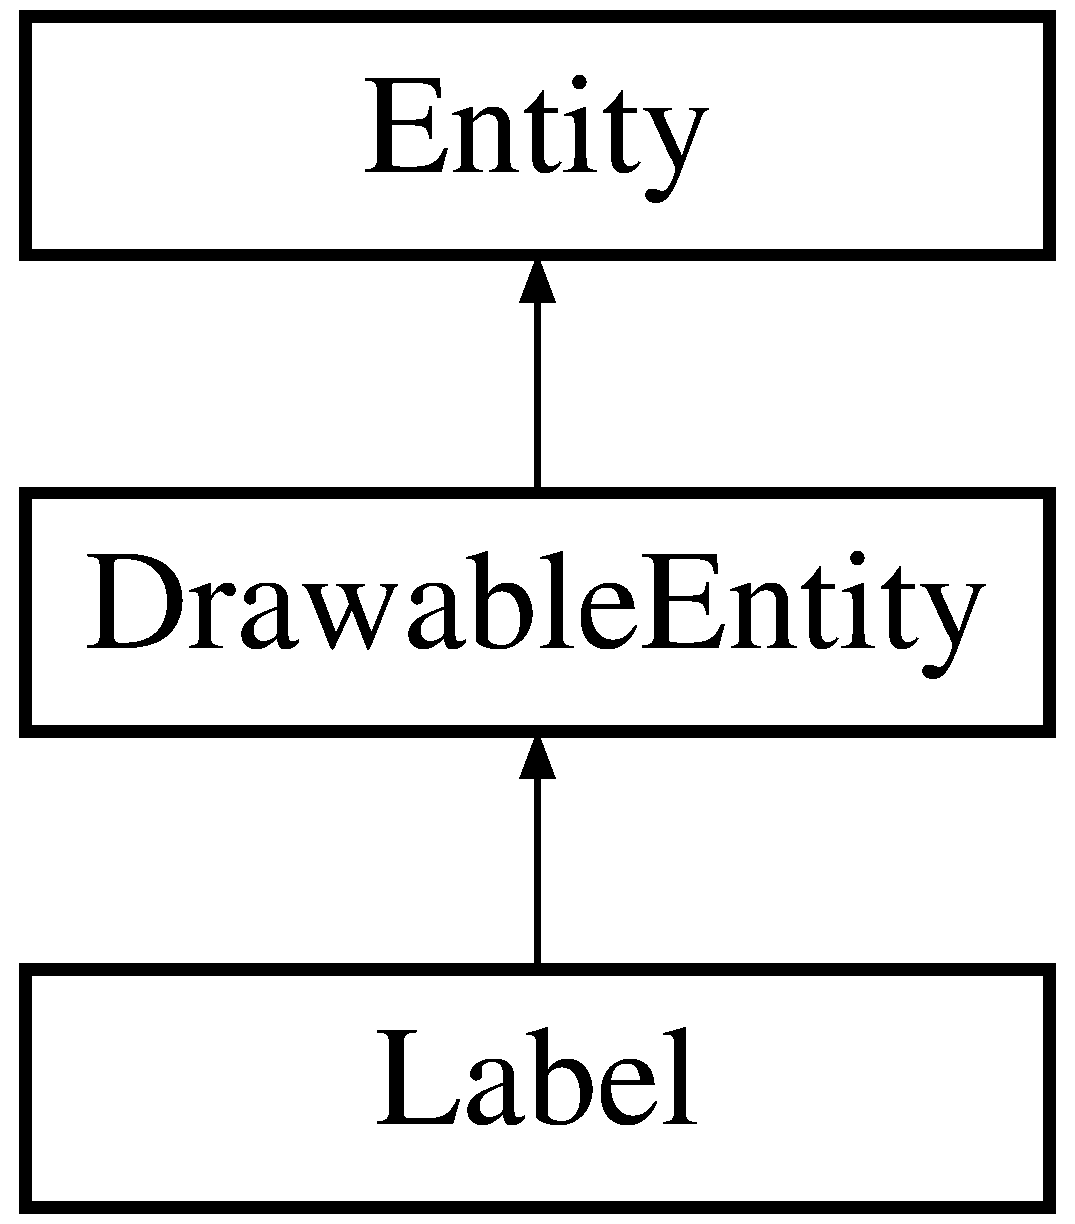
\includegraphics[height=3.000000cm]{class_label}
\end{center}
\end{figure}
\subsection*{Public Member Functions}
\begin{DoxyCompactItemize}
\item 
void \hyperlink{class_label_ab69dd0268124ac21d55b87734fd282a0}{init} (const uint8\+\_\+t r, const uint8\+\_\+t g, const uint8\+\_\+t b, const uint8\+\_\+t a, const float px, const float py, const float rotation, const float scalex, const float scaley, const char $\ast$text, const sf\+::\+Font \&font)
\item 
void \hyperlink{class_label_acaf5dfeeab3e46b5795b8cd24c9d94fe}{draw} (sf\+::\+Render\+Window \&window)
\item 
void \hyperlink{class_label_affe136b0a2e4a2240ecd30460222811d}{set\+\_\+font} (const sf\+::\+Font \&font)
\item 
void \hyperlink{class_label_a9e794358a782f0a4ba163bcbbe013612}{set\+\_\+font\+\_\+size} (const int32\+\_\+t \&font\+\_\+size)
\item 
bool \hyperlink{class_label_ad79f141fe2f04fd095b9507cac2667a6}{check\+Collision} (const sf\+::\+Vector2f \&position)
\item 
void \hyperlink{class_label_abafe12b2237df6f7e915d407d8084ec7}{unuse} ()
\end{DoxyCompactItemize}
\subsection*{Static Public Member Functions}
\begin{DoxyCompactItemize}
\item 
static \hyperlink{class_label}{Label} $\ast$ \hyperlink{class_label_a9331db7ea12bb0bfa69910b9aa2229a4}{Create\+Label} ()
\end{DoxyCompactItemize}
\subsection*{Public Attributes}
\begin{DoxyCompactItemize}
\item 
\mbox{\Hypertarget{class_label_a96bfd593e67f9031a244732fed63358f}\label{class_label_a96bfd593e67f9031a244732fed63358f}} 
int32\+\_\+t {\bfseries font\+\_\+size\+\_\+}
\item 
\mbox{\Hypertarget{class_label_a272e5426b0989b667b42cc4c87d697a7}\label{class_label_a272e5426b0989b667b42cc4c87d697a7}} 
char {\bfseries text\+\_\+} \mbox{[}k\+Text\+Max\+Size\mbox{]}
\item 
\mbox{\Hypertarget{class_label_a2f2da01fed83e50368d3d3674ed11d1b}\label{class_label_a2f2da01fed83e50368d3d3674ed11d1b}} 
sf\+::\+Text\+::\+Style {\bfseries style\+\_\+}
\item 
\mbox{\Hypertarget{class_label_a19110944dc9f96e238ca9e807d06421c}\label{class_label_a19110944dc9f96e238ca9e807d06421c}} 
const sf\+::\+Font $\ast$ {\bfseries font\+\_\+}
\end{DoxyCompactItemize}
\subsection*{Static Public Attributes}
\begin{DoxyCompactItemize}
\item 
\mbox{\Hypertarget{class_label_a00ba8c3c345de6f169c739243aad2634}\label{class_label_a00ba8c3c345de6f169c739243aad2634}} 
static const uint8\+\_\+t {\bfseries k\+Max\+Labels} = 50
\item 
\mbox{\Hypertarget{class_label_a73c9a955b95b4e3dfbba8b4a7771d64a}\label{class_label_a73c9a955b95b4e3dfbba8b4a7771d64a}} 
static const uint8\+\_\+t {\bfseries k\+Text\+Max\+Size} = 50
\end{DoxyCompactItemize}


\subsection{Detailed Description}
entity \hyperlink{class_label}{Label}

Class used to represent text. 

\subsection{Member Function Documentation}
\mbox{\Hypertarget{class_label_ad79f141fe2f04fd095b9507cac2667a6}\label{class_label_ad79f141fe2f04fd095b9507cac2667a6}} 
\index{Label@{Label}!check\+Collision@{check\+Collision}}
\index{check\+Collision@{check\+Collision}!Label@{Label}}
\subsubsection{\texorpdfstring{check\+Collision()}{checkCollision()}}
{\footnotesize\ttfamily bool Label\+::check\+Collision (\begin{DoxyParamCaption}\item[{const sf\+::\+Vector2f \&}]{position }\end{DoxyParamCaption})}

if a point collides with the label

Checks if the point passed by reference collides with the label.

\begin{DoxyReturn}{Returns}
bool returns true if the point collides and false if not. 
\end{DoxyReturn}
\mbox{\Hypertarget{class_label_a9331db7ea12bb0bfa69910b9aa2229a4}\label{class_label_a9331db7ea12bb0bfa69910b9aa2229a4}} 
\index{Label@{Label}!Create\+Label@{Create\+Label}}
\index{Create\+Label@{Create\+Label}!Label@{Label}}
\subsubsection{\texorpdfstring{Create\+Label()}{CreateLabel()}}
{\footnotesize\ttfamily static \hyperlink{class_label}{Label}$\ast$ Label\+::\+Create\+Label (\begin{DoxyParamCaption}{ }\end{DoxyParamCaption})\hspace{0.3cm}{\ttfamily [static]}}

that creates labels

Checks that the number of labels didn\textquotesingle{}t pass the maxim amount established If you wish to create a \hyperlink{class_label}{Label} you must use this method. In case the maximum amount of labels has been reached it will return nullptr. Otherwise it will return a pointer to a label.

\begin{DoxyReturn}{Returns}
Label$\ast$ returns the label created or nullptr if the maximum of labels has been reached 
\end{DoxyReturn}
\mbox{\Hypertarget{class_label_acaf5dfeeab3e46b5795b8cd24c9d94fe}\label{class_label_acaf5dfeeab3e46b5795b8cd24c9d94fe}} 
\index{Label@{Label}!draw@{draw}}
\index{draw@{draw}!Label@{Label}}
\subsubsection{\texorpdfstring{draw()}{draw()}}
{\footnotesize\ttfamily void Label\+::draw (\begin{DoxyParamCaption}\item[{sf\+::\+Render\+Window \&}]{window }\end{DoxyParamCaption})}

the graphic entity \hyperlink{class_label}{Label}

Draws the label using S\+F\+ML to the window passed by reference

\begin{DoxyReturn}{Returns}
void 
\end{DoxyReturn}

\begin{DoxyParams}{Parameters}
{\em window} & S\+F\+ML Render\+Window passed by reference \\
\hline
\end{DoxyParams}
\mbox{\Hypertarget{class_label_ab69dd0268124ac21d55b87734fd282a0}\label{class_label_ab69dd0268124ac21d55b87734fd282a0}} 
\index{Label@{Label}!init@{init}}
\index{init@{init}!Label@{Label}}
\subsubsection{\texorpdfstring{init()}{init()}}
{\footnotesize\ttfamily void Label\+::init (\begin{DoxyParamCaption}\item[{const uint8\+\_\+t}]{r,  }\item[{const uint8\+\_\+t}]{g,  }\item[{const uint8\+\_\+t}]{b,  }\item[{const uint8\+\_\+t}]{a,  }\item[{const float}]{px,  }\item[{const float}]{py,  }\item[{const float}]{rotation,  }\item[{const float}]{scalex,  }\item[{const float}]{scaley,  }\item[{const char $\ast$}]{text,  }\item[{const sf\+::\+Font \&}]{font }\end{DoxyParamCaption})}

the \hyperlink{class_label}{Label}

Initializes a label

\begin{DoxyReturn}{Returns}
void 
\end{DoxyReturn}

\begin{DoxyParams}{Parameters}
{\em r} & color red component of the label we want to create \\
\hline
{\em g} & color blue component of the label we want to create \\
\hline
{\em b} & color green component of the label we want to create \\
\hline
{\em a} & alpha channel of the color of the label we want to create \\
\hline
{\em px} & x position in the window \\
\hline
{\em py} & y position in the window \\
\hline
{\em rotation} & rotation in degrees \\
\hline
{\em scalex} & scale quantity at x axis \\
\hline
{\em scaley} & scale quantity at y axis \\
\hline
{\em text} & text that will contain the label \\
\hline
{\em font} & font of the text \\
\hline
\end{DoxyParams}
\mbox{\Hypertarget{class_label_affe136b0a2e4a2240ecd30460222811d}\label{class_label_affe136b0a2e4a2240ecd30460222811d}} 
\index{Label@{Label}!set\+\_\+font@{set\+\_\+font}}
\index{set\+\_\+font@{set\+\_\+font}!Label@{Label}}
\subsubsection{\texorpdfstring{set\+\_\+font()}{set\_font()}}
{\footnotesize\ttfamily void Label\+::set\+\_\+font (\begin{DoxyParamCaption}\item[{const sf\+::\+Font \&}]{font }\end{DoxyParamCaption})}

for text value

Changes the text value of the label

\begin{DoxyReturn}{Returns}
void 
\end{DoxyReturn}

\begin{DoxyParams}{Parameters}
{\em \&text} & reference to the new string we wish to show within the label \\
\hline
\end{DoxyParams}
\mbox{\Hypertarget{class_label_a9e794358a782f0a4ba163bcbbe013612}\label{class_label_a9e794358a782f0a4ba163bcbbe013612}} 
\index{Label@{Label}!set\+\_\+font\+\_\+size@{set\+\_\+font\+\_\+size}}
\index{set\+\_\+font\+\_\+size@{set\+\_\+font\+\_\+size}!Label@{Label}}
\subsubsection{\texorpdfstring{set\+\_\+font\+\_\+size()}{set\_font\_size()}}
{\footnotesize\ttfamily void Label\+::set\+\_\+font\+\_\+size (\begin{DoxyParamCaption}\item[{const int32\+\_\+t \&}]{font\+\_\+size }\end{DoxyParamCaption})}

for font\+\_\+size value

Changes the font size of the label

\begin{DoxyReturn}{Returns}
void 
\end{DoxyReturn}

\begin{DoxyParams}{Parameters}
{\em \&font\+\_\+size} & reference to the new font size of our label \\
\hline
\end{DoxyParams}
\mbox{\Hypertarget{class_label_abafe12b2237df6f7e915d407d8084ec7}\label{class_label_abafe12b2237df6f7e915d407d8084ec7}} 
\index{Label@{Label}!unuse@{unuse}}
\index{unuse@{unuse}!Label@{Label}}
\subsubsection{\texorpdfstring{unuse()}{unuse()}}
{\footnotesize\ttfamily void Label\+::unuse (\begin{DoxyParamCaption}{ }\end{DoxyParamCaption})}

the values of the label

Sets the attributes of the label to a default value to return it to a pool and being able to reuse it later.

\begin{DoxyReturn}{Returns}
void 
\end{DoxyReturn}


The documentation for this class was generated from the following file\+:\begin{DoxyCompactItemize}
\item 
2d\+\_\+engine/include/label.\+h\end{DoxyCompactItemize}

\hypertarget{class_native__dialogs}{}\section{Native\+\_\+dialogs Class Reference}
\label{class_native__dialogs}\index{Native\+\_\+dialogs@{Native\+\_\+dialogs}}
\subsection*{Public Member Functions}
\begin{DoxyCompactItemize}
\item 
void \hyperlink{class_native__dialogs_a325b62ac200ee9d8287a7320643d5385}{message\+Box} (const char $\ast$title, const char $\ast$message, const char $\ast$type, const char $\ast$icon, const int default\+Button)
\item 
const char $\ast$ \hyperlink{class_native__dialogs_a4bf815830a674dc34903d272391bcac3}{save\+File\+Dialog} (const char $\ast$title, const char $\ast$default\+File, const int num\+Of\+Filter\+Patterns, const char $\ast$$\ast$filter\+Patterns, const char $\ast$single\+Filter\+Description)
\item 
const char $\ast$ \hyperlink{class_native__dialogs_a57d8bdda43d74e367598bd5dc530b526}{open\+File\+Dialog} (const char $\ast$title, const char $\ast$default\+File, const int num\+Of\+Filter\+Patterns, const char $\ast$$\ast$filter\+Patterns, const char $\ast$single\+Filter\+Description)
\item 
const char $\ast$ \hyperlink{class_native__dialogs_a8bdf80cf55d1d5cf2835bc1b3e4084cc}{select\+Folder\+Dialog} (const char $\ast$title, const char $\ast$default\+Path)
\end{DoxyCompactItemize}


\subsection{Member Function Documentation}
\mbox{\Hypertarget{class_native__dialogs_a325b62ac200ee9d8287a7320643d5385}\label{class_native__dialogs_a325b62ac200ee9d8287a7320643d5385}} 
\index{Native\+\_\+dialogs@{Native\+\_\+dialogs}!message\+Box@{message\+Box}}
\index{message\+Box@{message\+Box}!Native\+\_\+dialogs@{Native\+\_\+dialogs}}
\subsubsection{\texorpdfstring{message\+Box()}{messageBox()}}
{\footnotesize\ttfamily void Native\+\_\+dialogs\+::message\+Box (\begin{DoxyParamCaption}\item[{const char $\ast$}]{title,  }\item[{const char $\ast$}]{message,  }\item[{const char $\ast$}]{type,  }\item[{const char $\ast$}]{icon,  }\item[{const int}]{default\+Button }\end{DoxyParamCaption})}

a message box native

Open a mesage box with the introduced message.

\begin{DoxyReturn}{Returns}
void 
\end{DoxyReturn}

\begin{DoxyParams}{Parameters}
{\em title} & Title of the message box \\
\hline
{\em message} & Message to write in the message box \\
\hline
{\em type} & Type of message box, can be\+: \char`\"{}ok\char`\"{}, \char`\"{}okcancel\char`\"{}, \char`\"{}yesno\char`\"{} or \char`\"{}yesnocancel\char`\"{} \\
\hline
{\em icon} & Icon to put in the message box, can be\+: \char`\"{}info\char`\"{} \char`\"{}warning\char`\"{} \char`\"{}error\char`\"{} or \char`\"{}question\char`\"{} \\
\hline
{\em default\+Button} & Default button\+: 0 for cancel/no, 1 for ok/yes or 2 for no in yesnocancel \\
\hline
\end{DoxyParams}
\mbox{\Hypertarget{class_native__dialogs_a57d8bdda43d74e367598bd5dc530b526}\label{class_native__dialogs_a57d8bdda43d74e367598bd5dc530b526}} 
\index{Native\+\_\+dialogs@{Native\+\_\+dialogs}!open\+File\+Dialog@{open\+File\+Dialog}}
\index{open\+File\+Dialog@{open\+File\+Dialog}!Native\+\_\+dialogs@{Native\+\_\+dialogs}}
\subsubsection{\texorpdfstring{open\+File\+Dialog()}{openFileDialog()}}
{\footnotesize\ttfamily const char$\ast$ Native\+\_\+dialogs\+::open\+File\+Dialog (\begin{DoxyParamCaption}\item[{const char $\ast$}]{title,  }\item[{const char $\ast$}]{default\+File,  }\item[{const int}]{num\+Of\+Filter\+Patterns,  }\item[{const char $\ast$$\ast$}]{filter\+Patterns,  }\item[{const char $\ast$}]{single\+Filter\+Description }\end{DoxyParamCaption})}

a open file dialog

Open a native dialog for open a file

\begin{DoxyReturn}{Returns}
void 
\end{DoxyReturn}

\begin{DoxyParams}{Parameters}
{\em title} & Title of the dialog box. Can be N\+U\+LL \\
\hline
{\em default\+File} & Put a default path and file to open. Can be N\+U\+LL. \\
\hline
{\em num\+Of\+Filter\+Patterns} & Number of posibles extensions to open. By default 0 \\
\hline
{\em filter\+Patterns} & Pattern with the posible extensions to open. i.\+e\+: \{\char`\"{}$\ast$.\+jpg\char`\"{},\char`\"{}$\ast$.\+png\char`\"{}\}. Can be N\+U\+LL \\
\hline
{\em single\+Filter\+Description} & Singl description of the file type \\
\hline
\end{DoxyParams}
\mbox{\Hypertarget{class_native__dialogs_a4bf815830a674dc34903d272391bcac3}\label{class_native__dialogs_a4bf815830a674dc34903d272391bcac3}} 
\index{Native\+\_\+dialogs@{Native\+\_\+dialogs}!save\+File\+Dialog@{save\+File\+Dialog}}
\index{save\+File\+Dialog@{save\+File\+Dialog}!Native\+\_\+dialogs@{Native\+\_\+dialogs}}
\subsubsection{\texorpdfstring{save\+File\+Dialog()}{saveFileDialog()}}
{\footnotesize\ttfamily const char$\ast$ Native\+\_\+dialogs\+::save\+File\+Dialog (\begin{DoxyParamCaption}\item[{const char $\ast$}]{title,  }\item[{const char $\ast$}]{default\+File,  }\item[{const int}]{num\+Of\+Filter\+Patterns,  }\item[{const char $\ast$$\ast$}]{filter\+Patterns,  }\item[{const char $\ast$}]{single\+Filter\+Description }\end{DoxyParamCaption})}

a save file dialog

Open a native dialog for save a file

\begin{DoxyReturn}{Returns}
void 
\end{DoxyReturn}

\begin{DoxyParams}{Parameters}
{\em title} & Title of the dialog box. Can be N\+U\+LL \\
\hline
{\em default\+File} & Put a default path and file to save. Can be N\+U\+LL. \\
\hline
{\em num\+Of\+Filter\+Patterns} & Number of posibles extensions to save. By default 0 \\
\hline
{\em filter\+Patterns} & Pattern with the posible extensions to save. i.\+e\+: \{\char`\"{}$\ast$.\+jpg\char`\"{},\char`\"{}$\ast$.\+png\char`\"{}\}. Can be N\+U\+LL \\
\hline
{\em single\+Filter\+Description} & Singl description of the file type \\
\hline
\end{DoxyParams}
\mbox{\Hypertarget{class_native__dialogs_a8bdf80cf55d1d5cf2835bc1b3e4084cc}\label{class_native__dialogs_a8bdf80cf55d1d5cf2835bc1b3e4084cc}} 
\index{Native\+\_\+dialogs@{Native\+\_\+dialogs}!select\+Folder\+Dialog@{select\+Folder\+Dialog}}
\index{select\+Folder\+Dialog@{select\+Folder\+Dialog}!Native\+\_\+dialogs@{Native\+\_\+dialogs}}
\subsubsection{\texorpdfstring{select\+Folder\+Dialog()}{selectFolderDialog()}}
{\footnotesize\ttfamily const char$\ast$ Native\+\_\+dialogs\+::select\+Folder\+Dialog (\begin{DoxyParamCaption}\item[{const char $\ast$}]{title,  }\item[{const char $\ast$}]{default\+Path }\end{DoxyParamCaption})}

a select folder dialog

Open a native dialog for select a folder

\begin{DoxyReturn}{Returns}
void 
\end{DoxyReturn}

\begin{DoxyParams}{Parameters}
{\em title} & Title of the dialog box. Can be N\+U\+LL \\
\hline
{\em default\+Path} & Put a default path to open. Can be N\+U\+LL. \\
\hline
\end{DoxyParams}


The documentation for this class was generated from the following file\+:\begin{DoxyCompactItemize}
\item 
include/native\+\_\+dialogs.\+h\end{DoxyCompactItemize}

\hypertarget{class_pool}{}\section{Pool Class Reference}
\label{class_pool}\index{Pool@{Pool}}


{\ttfamily \#include $<$pool.\+h$>$}

\subsection*{Public Member Functions}
\begin{DoxyCompactItemize}
\item 
void \hyperlink{class_pool_a7b5bfb074b19ea0169edf7c2d73b2f6e}{init} ()
\item 
void \hyperlink{class_pool_aa2bcc7b11c5f0a438b1fe5405ba698ff}{free} ()
\item 
\hyperlink{class_rect}{Rect} $\ast$ \hyperlink{class_pool_a2ea49e227ce14fcb926d451f9f59e452}{get\+Rect} ()
\item 
\hyperlink{class_label}{Label} $\ast$ \hyperlink{class_pool_a13ce02d7dbee29305a83dcdb22a01661}{get\+Label} ()
\item 
\hyperlink{class_sprite}{Sprite} $\ast$ \hyperlink{class_pool_abd15708186d45b2e45312c872dd84384}{get\+Sprite} ()
\item 
\hyperlink{class_background}{Background} $\ast$ \hyperlink{class_pool_a367c875efe93a27fea4bcaf0ed281abd}{get\+Background} ()
\item 
void \hyperlink{class_pool_a3b5250c08babf163d9d4877c7a2a6f40}{return\+Rect} (\hyperlink{class_rect}{Rect} \&rect)
\item 
void \hyperlink{class_pool_a2a38a2d1aa883152d27fa213ac2cc2e8}{return\+Label} (\hyperlink{class_label}{Label} \&label)
\item 
void \hyperlink{class_pool_a227334c0983a0c1bf42d72a44fcfee8f}{return\+Sprite} (\hyperlink{class_sprite}{Sprite} \&sprite)
\item 
void \hyperlink{class_pool_af6234b218a3dd72a440a3381b35c9e36}{return\+Background} (\hyperlink{class_background}{Background} \&background)
\end{DoxyCompactItemize}
\subsection*{Static Public Member Functions}
\begin{DoxyCompactItemize}
\item 
static \hyperlink{class_pool}{Pool} \& \hyperlink{class_pool_a20e44e0054d4eedf57f1943b87c06e20}{instance} ()
\end{DoxyCompactItemize}
\subsection*{Public Attributes}
\begin{DoxyCompactItemize}
\item 
\mbox{\Hypertarget{class_pool_a2a73ee4005262cd6f4ebfc25a1811fce}\label{class_pool_a2a73ee4005262cd6f4ebfc25a1811fce}} 
std\+::vector$<$ \hyperlink{class_rect}{Rect} $\ast$ $>$ {\bfseries rect\+\_\+pool\+\_\+}
\item 
\mbox{\Hypertarget{class_pool_a5ea3bbd258fcb452dcfa036ac5acacd5}\label{class_pool_a5ea3bbd258fcb452dcfa036ac5acacd5}} 
std\+::vector$<$ \hyperlink{class_label}{Label} $\ast$ $>$ {\bfseries label\+\_\+pool\+\_\+}
\item 
\mbox{\Hypertarget{class_pool_a0bd32066fb5351695261a6fa1f1796bf}\label{class_pool_a0bd32066fb5351695261a6fa1f1796bf}} 
std\+::vector$<$ \hyperlink{class_sprite}{Sprite} $\ast$ $>$ {\bfseries sprite\+\_\+pool\+\_\+}
\item 
\mbox{\Hypertarget{class_pool_a11e4e7ab2e2d9307e7ec5dd56ffc84ed}\label{class_pool_a11e4e7ab2e2d9307e7ec5dd56ffc84ed}} 
std\+::vector$<$ \hyperlink{class_background}{Background} $\ast$ $>$ {\bfseries bg\+\_\+pool\+\_\+}
\end{DoxyCompactItemize}


\subsection{Detailed Description}
in charge of managing the pools

Singleton of pools used to reuse the diverse graphical entities of the application avoiding this way the destruction of objects during execution as much as possible 

\subsection{Member Function Documentation}
\mbox{\Hypertarget{class_pool_aa2bcc7b11c5f0a438b1fe5405ba698ff}\label{class_pool_aa2bcc7b11c5f0a438b1fe5405ba698ff}} 
\index{Pool@{Pool}!free@{free}}
\index{free@{free}!Pool@{Pool}}
\subsubsection{\texorpdfstring{free()}{free()}}
{\footnotesize\ttfamily void Pool\+::free (\begin{DoxyParamCaption}{ }\end{DoxyParamCaption})}

the pull

Frees all the elements stored in the pools.

\begin{DoxyReturn}{Returns}
void 
\end{DoxyReturn}
\mbox{\Hypertarget{class_pool_a367c875efe93a27fea4bcaf0ed281abd}\label{class_pool_a367c875efe93a27fea4bcaf0ed281abd}} 
\index{Pool@{Pool}!get\+Background@{get\+Background}}
\index{get\+Background@{get\+Background}!Pool@{Pool}}
\subsubsection{\texorpdfstring{get\+Background()}{getBackground()}}
{\footnotesize\ttfamily \hyperlink{class_background}{Background}$\ast$ Pool\+::get\+Background (\begin{DoxyParamCaption}{ }\end{DoxyParamCaption})}

a \hyperlink{class_background}{Background}

Returns a \hyperlink{class_background}{Background} from the pool, if the pool doesn\textquotesingle{}t have more backgrounds it creates one using the background factory. If the max of backgrounds has been reached it returns null ptr.

\begin{DoxyReturn}{Returns}
Background$\ast$ pointer to background if possible, nullptr if the maxim has been reached 
\end{DoxyReturn}
\mbox{\Hypertarget{class_pool_a13ce02d7dbee29305a83dcdb22a01661}\label{class_pool_a13ce02d7dbee29305a83dcdb22a01661}} 
\index{Pool@{Pool}!get\+Label@{get\+Label}}
\index{get\+Label@{get\+Label}!Pool@{Pool}}
\subsubsection{\texorpdfstring{get\+Label()}{getLabel()}}
{\footnotesize\ttfamily \hyperlink{class_label}{Label}$\ast$ Pool\+::get\+Label (\begin{DoxyParamCaption}{ }\end{DoxyParamCaption})}

a \hyperlink{class_label}{Label}

Returns a \hyperlink{class_label}{Label} from the pool, if the pool doesn\textquotesingle{}t have more labels it creates one using the label factory. If the max of labels has been reached it returns null ptr.

\begin{DoxyReturn}{Returns}
Label$\ast$ pointer to label if possible, nullptr if the maxim has been reached 
\end{DoxyReturn}
\mbox{\Hypertarget{class_pool_a2ea49e227ce14fcb926d451f9f59e452}\label{class_pool_a2ea49e227ce14fcb926d451f9f59e452}} 
\index{Pool@{Pool}!get\+Rect@{get\+Rect}}
\index{get\+Rect@{get\+Rect}!Pool@{Pool}}
\subsubsection{\texorpdfstring{get\+Rect()}{getRect()}}
{\footnotesize\ttfamily \hyperlink{class_rect}{Rect}$\ast$ Pool\+::get\+Rect (\begin{DoxyParamCaption}{ }\end{DoxyParamCaption})}

a \hyperlink{class_rect}{Rect}

Returns a \hyperlink{class_rect}{Rect} from the pool, if the pool doesn\textquotesingle{}t have more rects it creates one using the rect factory. If the max of rects has been reached it returns null ptr.

\begin{DoxyReturn}{Returns}
Rect$\ast$ pointer to rect if possible, nullptr if the maxim has been reached 
\end{DoxyReturn}
\mbox{\Hypertarget{class_pool_abd15708186d45b2e45312c872dd84384}\label{class_pool_abd15708186d45b2e45312c872dd84384}} 
\index{Pool@{Pool}!get\+Sprite@{get\+Sprite}}
\index{get\+Sprite@{get\+Sprite}!Pool@{Pool}}
\subsubsection{\texorpdfstring{get\+Sprite()}{getSprite()}}
{\footnotesize\ttfamily \hyperlink{class_sprite}{Sprite}$\ast$ Pool\+::get\+Sprite (\begin{DoxyParamCaption}{ }\end{DoxyParamCaption})}

a \hyperlink{class_sprite}{Sprite}

Returns a \hyperlink{class_sprite}{Sprite} from the pool, if the pool doesn\textquotesingle{}t have more sprites it creates one using the sprite factory. If the max of sprites has been reached it returns null ptr.

\begin{DoxyReturn}{Returns}
Sprite$\ast$ pointer to sprite if possible, nullptr if the maxim has been reached 
\end{DoxyReturn}
\mbox{\Hypertarget{class_pool_a7b5bfb074b19ea0169edf7c2d73b2f6e}\label{class_pool_a7b5bfb074b19ea0169edf7c2d73b2f6e}} 
\index{Pool@{Pool}!init@{init}}
\index{init@{init}!Pool@{Pool}}
\subsubsection{\texorpdfstring{init()}{init()}}
{\footnotesize\ttfamily void Pool\+::init (\begin{DoxyParamCaption}{ }\end{DoxyParamCaption})}

the pool

Initializes the pool creating the first instances of the elements.

\begin{DoxyReturn}{Returns}
void 
\end{DoxyReturn}
\mbox{\Hypertarget{class_pool_a20e44e0054d4eedf57f1943b87c06e20}\label{class_pool_a20e44e0054d4eedf57f1943b87c06e20}} 
\index{Pool@{Pool}!instance@{instance}}
\index{instance@{instance}!Pool@{Pool}}
\subsubsection{\texorpdfstring{instance()}{instance()}}
{\footnotesize\ttfamily static \hyperlink{class_pool}{Pool}\& Pool\+::instance (\begin{DoxyParamCaption}{ }\end{DoxyParamCaption})\hspace{0.3cm}{\ttfamily [static]}}

the instance of our pool

In charge of creating our singleton of pools in case it doesn\textquotesingle{}t exist or return it\textquotesingle{}s instance if it exists.

\begin{DoxyReturn}{Returns}
\hyperlink{class_pool}{Pool}\& instance of the pool 
\end{DoxyReturn}
\mbox{\Hypertarget{class_pool_af6234b218a3dd72a440a3381b35c9e36}\label{class_pool_af6234b218a3dd72a440a3381b35c9e36}} 
\index{Pool@{Pool}!return\+Background@{return\+Background}}
\index{return\+Background@{return\+Background}!Pool@{Pool}}
\subsubsection{\texorpdfstring{return\+Background()}{returnBackground()}}
{\footnotesize\ttfamily void Pool\+::return\+Background (\begin{DoxyParamCaption}\item[{\hyperlink{class_background}{Background} \&}]{background }\end{DoxyParamCaption})}

an existing background to the pool

Recieves an existing background and resets it\textquotesingle{}s value using the unuse function of background

\begin{DoxyReturn}{Returns}
void 
\end{DoxyReturn}
\mbox{\Hypertarget{class_pool_a2a38a2d1aa883152d27fa213ac2cc2e8}\label{class_pool_a2a38a2d1aa883152d27fa213ac2cc2e8}} 
\index{Pool@{Pool}!return\+Label@{return\+Label}}
\index{return\+Label@{return\+Label}!Pool@{Pool}}
\subsubsection{\texorpdfstring{return\+Label()}{returnLabel()}}
{\footnotesize\ttfamily void Pool\+::return\+Label (\begin{DoxyParamCaption}\item[{\hyperlink{class_label}{Label} \&}]{label }\end{DoxyParamCaption})}

an existing label to the pool

Recieves an existing label and resets it\textquotesingle{}s value using the unuse function of label

\begin{DoxyReturn}{Returns}
void 
\end{DoxyReturn}
\mbox{\Hypertarget{class_pool_a3b5250c08babf163d9d4877c7a2a6f40}\label{class_pool_a3b5250c08babf163d9d4877c7a2a6f40}} 
\index{Pool@{Pool}!return\+Rect@{return\+Rect}}
\index{return\+Rect@{return\+Rect}!Pool@{Pool}}
\subsubsection{\texorpdfstring{return\+Rect()}{returnRect()}}
{\footnotesize\ttfamily void Pool\+::return\+Rect (\begin{DoxyParamCaption}\item[{\hyperlink{class_rect}{Rect} \&}]{rect }\end{DoxyParamCaption})}

an existing rect to the pool

Recieves an existing rect and resets it\textquotesingle{}s value using the unuse function of rect

\begin{DoxyReturn}{Returns}
void 
\end{DoxyReturn}
\mbox{\Hypertarget{class_pool_a227334c0983a0c1bf42d72a44fcfee8f}\label{class_pool_a227334c0983a0c1bf42d72a44fcfee8f}} 
\index{Pool@{Pool}!return\+Sprite@{return\+Sprite}}
\index{return\+Sprite@{return\+Sprite}!Pool@{Pool}}
\subsubsection{\texorpdfstring{return\+Sprite()}{returnSprite()}}
{\footnotesize\ttfamily void Pool\+::return\+Sprite (\begin{DoxyParamCaption}\item[{\hyperlink{class_sprite}{Sprite} \&}]{sprite }\end{DoxyParamCaption})}

an existing sprite to the pool

Recieves an existing sprite and resets it\textquotesingle{}s value using the unuse function of sprite

\begin{DoxyReturn}{Returns}
void 
\end{DoxyReturn}


The documentation for this class was generated from the following file\+:\begin{DoxyCompactItemize}
\item 
2d\+\_\+engine/include/pool.\+h\end{DoxyCompactItemize}

\hypertarget{class_rect}{}\section{Rect Class Reference}
\label{class_rect}\index{Rect@{Rect}}


{\ttfamily \#include $<$rect.\+h$>$}

Inheritance diagram for Rect\+:\begin{figure}[H]
\begin{center}
\leavevmode
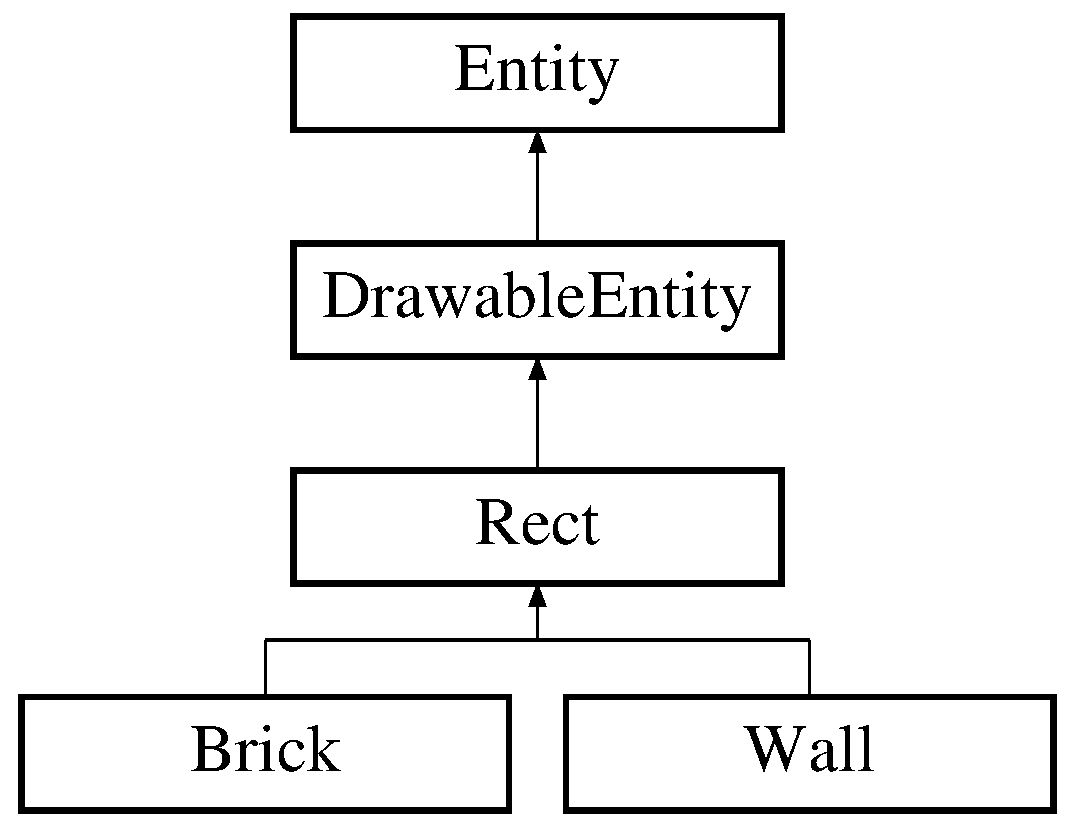
\includegraphics[height=3.000000cm]{class_rect}
\end{center}
\end{figure}
\subsection*{Public Member Functions}
\begin{DoxyCompactItemize}
\item 
void \hyperlink{class_rect_aa780623e4639a2679ed300424142d50d}{init} (uint8\+\_\+t is\+\_\+solid, float width, float height, uint8\+\_\+t sc\+\_\+r, uint8\+\_\+t sc\+\_\+g, uint8\+\_\+t sc\+\_\+b, uint8\+\_\+t sc\+\_\+a, uint8\+\_\+t fc\+\_\+r, uint8\+\_\+t fc\+\_\+g, uint8\+\_\+t fc\+\_\+b, uint8\+\_\+t fc\+\_\+a, float px, float py, float rotation, float scalex, float scaley)
\item 
void \hyperlink{class_rect_aa131d780f6ebb75e9057c01221486adc}{draw} (sf\+::\+Render\+Window \&window)
\item 
void \hyperlink{class_rect_ab7593e78f2fbc2354d8ef832ac3625a7}{resize} (const float width, const float height)
\item 
bool \hyperlink{class_rect_afb4fd23ac0ebf55ef7d9c1bcdcc7ff30}{check\+Collision} (const sf\+::\+Vector2f \&position)
\item 
void \hyperlink{class_rect_a31c7cbadb97080dfb559f3d04acc0bc9}{unuse} ()
\end{DoxyCompactItemize}
\subsection*{Static Public Member Functions}
\begin{DoxyCompactItemize}
\item 
static \hyperlink{class_rect}{Rect} $\ast$ \hyperlink{class_rect_ac9283327c926d453d0cd5a49ded8d150}{Create\+Rect} ()
\end{DoxyCompactItemize}
\subsection*{Public Attributes}
\begin{DoxyCompactItemize}
\item 
\mbox{\Hypertarget{class_rect_a898ebf0731c53c824582d4b1930b9e90}\label{class_rect_a898ebf0731c53c824582d4b1930b9e90}} 
uint8\+\_\+t {\bfseries is\+\_\+solid\+\_\+}
\item 
\mbox{\Hypertarget{class_rect_abb92a0e14f750712887e2061866a52bd}\label{class_rect_abb92a0e14f750712887e2061866a52bd}} 
sf\+::\+Vector2f {\bfseries dimensions\+\_\+}
\item 
\mbox{\Hypertarget{class_rect_a6af011eb6f16dabee8eff47e0772260e}\label{class_rect_a6af011eb6f16dabee8eff47e0772260e}} 
sf\+::\+Color {\bfseries rgba\+\_\+fill\+\_\+}
\end{DoxyCompactItemize}
\subsection*{Static Public Attributes}
\begin{DoxyCompactItemize}
\item 
\mbox{\Hypertarget{class_rect_a18981822ae235d9ed80b6dd9ba257fcc}\label{class_rect_a18981822ae235d9ed80b6dd9ba257fcc}} 
static const uint8\+\_\+t {\bfseries k\+Max\+Rects} = 50
\end{DoxyCompactItemize}


\subsection{Detailed Description}
entity \hyperlink{class_label}{Label}

Class used to represent Rectangles. 

\subsection{Member Function Documentation}
\mbox{\Hypertarget{class_rect_afb4fd23ac0ebf55ef7d9c1bcdcc7ff30}\label{class_rect_afb4fd23ac0ebf55ef7d9c1bcdcc7ff30}} 
\index{Rect@{Rect}!check\+Collision@{check\+Collision}}
\index{check\+Collision@{check\+Collision}!Rect@{Rect}}
\subsubsection{\texorpdfstring{check\+Collision()}{checkCollision()}}
{\footnotesize\ttfamily bool Rect\+::check\+Collision (\begin{DoxyParamCaption}\item[{const sf\+::\+Vector2f \&}]{position }\end{DoxyParamCaption})}

if a point collides with the rect

Checks if the point passed by reference collides with the rect.

\begin{DoxyReturn}{Returns}
bool returns true if the point collides and false if not. 
\end{DoxyReturn}
\mbox{\Hypertarget{class_rect_ac9283327c926d453d0cd5a49ded8d150}\label{class_rect_ac9283327c926d453d0cd5a49ded8d150}} 
\index{Rect@{Rect}!Create\+Rect@{Create\+Rect}}
\index{Create\+Rect@{Create\+Rect}!Rect@{Rect}}
\subsubsection{\texorpdfstring{Create\+Rect()}{CreateRect()}}
{\footnotesize\ttfamily static \hyperlink{class_rect}{Rect}$\ast$ Rect\+::\+Create\+Rect (\begin{DoxyParamCaption}{ }\end{DoxyParamCaption})\hspace{0.3cm}{\ttfamily [static]}}

that creates rect

Checks that the number of rects didn\textquotesingle{}t pass the maxim amount established If you wish to create a \hyperlink{class_rect}{Rect} you must use this method. In case the maximum amount of rects has been reached it will return nullptr. Otherwise it will return a pointer to a rect.

\begin{DoxyReturn}{Returns}
Rect$\ast$ returns the rect created or nullptr if the maximum of rects has been reached 
\end{DoxyReturn}
\mbox{\Hypertarget{class_rect_aa131d780f6ebb75e9057c01221486adc}\label{class_rect_aa131d780f6ebb75e9057c01221486adc}} 
\index{Rect@{Rect}!draw@{draw}}
\index{draw@{draw}!Rect@{Rect}}
\subsubsection{\texorpdfstring{draw()}{draw()}}
{\footnotesize\ttfamily void Rect\+::draw (\begin{DoxyParamCaption}\item[{sf\+::\+Render\+Window \&}]{window }\end{DoxyParamCaption})}

the graphic entity Rectangle

Draws the rectangle using S\+F\+ML to the window passed by reference

\begin{DoxyReturn}{Returns}
void 
\end{DoxyReturn}

\begin{DoxyParams}{Parameters}
{\em window} & S\+F\+ML Render\+Window passed by reference \\
\hline
\end{DoxyParams}
\mbox{\Hypertarget{class_rect_aa780623e4639a2679ed300424142d50d}\label{class_rect_aa780623e4639a2679ed300424142d50d}} 
\index{Rect@{Rect}!init@{init}}
\index{init@{init}!Rect@{Rect}}
\subsubsection{\texorpdfstring{init()}{init()}}
{\footnotesize\ttfamily void Rect\+::init (\begin{DoxyParamCaption}\item[{uint8\+\_\+t}]{is\+\_\+solid,  }\item[{float}]{width,  }\item[{float}]{height,  }\item[{uint8\+\_\+t}]{sc\+\_\+r,  }\item[{uint8\+\_\+t}]{sc\+\_\+g,  }\item[{uint8\+\_\+t}]{sc\+\_\+b,  }\item[{uint8\+\_\+t}]{sc\+\_\+a,  }\item[{uint8\+\_\+t}]{fc\+\_\+r,  }\item[{uint8\+\_\+t}]{fc\+\_\+g,  }\item[{uint8\+\_\+t}]{fc\+\_\+b,  }\item[{uint8\+\_\+t}]{fc\+\_\+a,  }\item[{float}]{px,  }\item[{float}]{py,  }\item[{float}]{rotation,  }\item[{float}]{scalex,  }\item[{float}]{scaley }\end{DoxyParamCaption})}

the \hyperlink{class_rect}{Rect}

Initializes the different values of a rect

\begin{DoxyReturn}{Returns}
void 
\end{DoxyReturn}

\begin{DoxyParams}{Parameters}
{\em is\+\_\+solid} & used to indicate if the rect has fill color \\
\hline
{\em width} & width dimension of the rectangle \\
\hline
{\em height} & height dimension of the rectangle \\
\hline
{\em sc\+\_\+r} & color red component of the inner color \\
\hline
{\em sc\+\_\+g} & color blue component of the inner color \\
\hline
{\em sc\+\_\+b} & color green component of the inner color \\
\hline
{\em sc\+\_\+a} & alpha channel of the inner color \\
\hline
{\em fc\+\_\+r} & color red component of the fill color \\
\hline
{\em fc\+\_\+g} & color blue component of the fill color \\
\hline
{\em fc\+\_\+b} & color green component of the fill color \\
\hline
{\em fc\+\_\+a} & alpha channel of the fill color \\
\hline
{\em px} & x position in the window \\
\hline
{\em py} & y position in the window \\
\hline
{\em rotation} & rotation in degrees \\
\hline
{\em scalex} & scale quantity at x axis \\
\hline
{\em scaley} & scale quantity at y axis \\
\hline
\end{DoxyParams}
\mbox{\Hypertarget{class_rect_ab7593e78f2fbc2354d8ef832ac3625a7}\label{class_rect_ab7593e78f2fbc2354d8ef832ac3625a7}} 
\index{Rect@{Rect}!resize@{resize}}
\index{resize@{resize}!Rect@{Rect}}
\subsubsection{\texorpdfstring{resize()}{resize()}}
{\footnotesize\ttfamily void Rect\+::resize (\begin{DoxyParamCaption}\item[{const float}]{width,  }\item[{const float}]{height }\end{DoxyParamCaption})}

the size of the rect

Sets the value of width and height for the rect to the ones indicated by parameter.

new width of the rectangle  new height of the rectangle \mbox{\Hypertarget{class_rect_a31c7cbadb97080dfb559f3d04acc0bc9}\label{class_rect_a31c7cbadb97080dfb559f3d04acc0bc9}} 
\index{Rect@{Rect}!unuse@{unuse}}
\index{unuse@{unuse}!Rect@{Rect}}
\subsubsection{\texorpdfstring{unuse()}{unuse()}}
{\footnotesize\ttfamily void Rect\+::unuse (\begin{DoxyParamCaption}{ }\end{DoxyParamCaption})}

the values of the rect

Sets the attributes of the rect to a default value to return it to a pool and being able to reuse it later.

\begin{DoxyReturn}{Returns}
void 
\end{DoxyReturn}


The documentation for this class was generated from the following file\+:\begin{DoxyCompactItemize}
\item 
2d\+\_\+engine/include/rect.\+h\end{DoxyCompactItemize}

\hypertarget{class_scene}{}\section{Scene Class Reference}
\label{class_scene}\index{Scene@{Scene}}


{\ttfamily \#include $<$scene.\+h$>$}

\subsection*{Public Member Functions}
\begin{DoxyCompactItemize}
\item 
void \hyperlink{class_scene_a6c4a04bd6fb848a1bdf8d1a82792c1ef}{clean\+Scene} ()
\item 
void \hyperlink{class_scene_aca9bd4059c420909135294125b591682}{load\+Scene} (const std\+::string scene\+\_\+path, const sf\+::\+Font \&font)
\item 
void \hyperlink{class_scene_a70c218eb67b3507a56486e1dd945f095}{save\+Scene} (const std\+::string scene\+\_\+path)
\item 
void \hyperlink{class_scene_a07d6d13ed45e8882192bed7330e5383a}{add\+Background} (\hyperlink{class_background}{Background} \&background)
\item 
\hyperlink{class_background}{Background} $\ast$ \hyperlink{class_scene_ade83d8b5c8b13f12b11c9ef07507163d}{get\+Background} (const uint32\+\_\+t background\+\_\+id)
\item 
void \hyperlink{class_scene_a33e4cfa3d8433c5ccb8842ca65d85c70}{remove\+Background} (const uint32\+\_\+t background\+\_\+id)
\item 
void \hyperlink{class_scene_a95b1dd31805e0734f66fb9f131166fa4}{change\+Z\+Order\+Background} (const uint32\+\_\+t background\+\_\+id, const int32\+\_\+t new\+Z\+Order)
\item 
void \hyperlink{class_scene_a2ef42ab154353fa7881f9f7382f43b1f}{add\+Rect} (\hyperlink{class_rect}{Rect} \&rect)
\item 
\hyperlink{class_rect}{Rect} $\ast$ \hyperlink{class_scene_abff9132084e8edf5eee4f992233dc2e3}{get\+Rect} (const uint32\+\_\+t rect\+\_\+id)
\item 
void \hyperlink{class_scene_a1e0fa3c3898c30822e14fdaa963eaa62}{remove\+Rect} (const uint32\+\_\+t rect\+\_\+id)
\item 
void \hyperlink{class_scene_aee2976ddb158bde51704f40cf0266e10}{change\+Z\+Order\+Rect} (const uint32\+\_\+t rect\+\_\+id, const int32\+\_\+t new\+Z\+Order)
\item 
void \hyperlink{class_scene_a4327310c11ae2f3130ddb61ed20cfda3}{add\+Label} (\hyperlink{class_label}{Label} \&label)
\item 
\hyperlink{class_label}{Label} $\ast$ \hyperlink{class_scene_aa65487dbbc075503ccf386df47b5cbc8}{get\+Label} (const uint32\+\_\+t label\+\_\+id)
\item 
void \hyperlink{class_scene_ac8e9f99810684c6bd397477972691cb8}{remove\+Label} (const uint32\+\_\+t label\+\_\+id)
\item 
void \hyperlink{class_scene_ac7dc181963c83afe8d3863e4226a3bd2}{change\+Z\+Order\+Label} (const uint32\+\_\+t label\+\_\+id, const int32\+\_\+t new\+Z\+Order)
\item 
void \hyperlink{class_scene_ac7bada9fa9ea8dbeee358693b44e540e}{add\+Sprite} (\hyperlink{class_sprite}{Sprite} \&sprite)
\item 
\hyperlink{class_sprite}{Sprite} $\ast$ \hyperlink{class_scene_a45418063b55b68e440cac7fab52e3c51}{get\+Sprite} (const uint32\+\_\+t sprite\+\_\+id)
\item 
void \hyperlink{class_scene_a6033b04f27e305069727d210e86b3902}{remove\+Sprite} (const uint32\+\_\+t sprite\+\_\+id)
\item 
void \hyperlink{class_scene_a3913b5c955c938f6bbd84d3e78bebcad}{change\+Z\+Order\+Sprite} (const uint32\+\_\+t sprite\+\_\+id, const int32\+\_\+t new\+Z\+Order)
\item 
void \hyperlink{class_scene_ad7c686656e9ad8e20f85f7997c4bc747}{add\+Texture} (sf\+::\+Texture \&texture, const std\+::string texture\+\_\+path)
\begin{DoxyCompactList}\small\item\em Texture ///. \end{DoxyCompactList}\item 
sf\+::\+Texture $\ast$ \hyperlink{class_scene_a1c7233bcc955b7b71156b31205ec2360}{get\+Texture} (const std\+::string texture\+\_\+path)
\item 
void \hyperlink{class_scene_a6418fa4353c7d079b42e11af7343c8a9}{remove\+Texture} (const std\+::string texture\+\_\+path)
\item 
uint32\+\_\+t \hyperlink{class_scene_a8a29c60fda35f60e0d2ab54b497955ec}{check\+Collision} (sf\+::\+Vector2f \&position, uint8\+\_\+t $\ast$type)
\item 
std\+::list$<$ \hyperlink{class_drawable_entity}{Drawable\+Entity} $\ast$ $>$ \hyperlink{class_scene_a53baaa91f1356e5fe9abc9b5a1cffb94}{get\+Drawable\+Entities\+By\+Tag} (const uint32\+\_\+t tag)
\item 
void \hyperlink{class_scene_ae27f4327ca363cc9cad8ab553504e2d5}{draw\+Scene} ()
\item 
void \hyperlink{class_scene_aa24c7e636c10e4e42650c1374b90bb80}{update} ()
\end{DoxyCompactItemize}


\subsection{Detailed Description}
Class that create and manage a scene

This class create and manage the scene and all the elements that form it. 

\subsection{Member Function Documentation}
\mbox{\Hypertarget{class_scene_a07d6d13ed45e8882192bed7330e5383a}\label{class_scene_a07d6d13ed45e8882192bed7330e5383a}} 
\index{Scene@{Scene}!add\+Background@{add\+Background}}
\index{add\+Background@{add\+Background}!Scene@{Scene}}
\subsubsection{\texorpdfstring{add\+Background()}{addBackground()}}
{\footnotesize\ttfamily void Scene\+::add\+Background (\begin{DoxyParamCaption}\item[{\hyperlink{class_background}{Background} \&}]{background }\end{DoxyParamCaption})}

a \hyperlink{class_background}{Background} to the scene

Add a \hyperlink{class_background}{Background} in the mappings that form the scene

\begin{DoxyReturn}{Returns}
void 
\end{DoxyReturn}

\begin{DoxyParams}{Parameters}
{\em background} & Reference of the \hyperlink{class_background}{Background} to add \\
\hline
\end{DoxyParams}
\mbox{\Hypertarget{class_scene_a4327310c11ae2f3130ddb61ed20cfda3}\label{class_scene_a4327310c11ae2f3130ddb61ed20cfda3}} 
\index{Scene@{Scene}!add\+Label@{add\+Label}}
\index{add\+Label@{add\+Label}!Scene@{Scene}}
\subsubsection{\texorpdfstring{add\+Label()}{addLabel()}}
{\footnotesize\ttfamily void Scene\+::add\+Label (\begin{DoxyParamCaption}\item[{\hyperlink{class_label}{Label} \&}]{label }\end{DoxyParamCaption})}

a \hyperlink{class_label}{Label} to the scene

Add a \hyperlink{class_label}{Label} in the mappings that form the scene

\begin{DoxyReturn}{Returns}
void 
\end{DoxyReturn}

\begin{DoxyParams}{Parameters}
{\em label} & Reference of the \hyperlink{class_label}{Label} to add \\
\hline
\end{DoxyParams}
\mbox{\Hypertarget{class_scene_a2ef42ab154353fa7881f9f7382f43b1f}\label{class_scene_a2ef42ab154353fa7881f9f7382f43b1f}} 
\index{Scene@{Scene}!add\+Rect@{add\+Rect}}
\index{add\+Rect@{add\+Rect}!Scene@{Scene}}
\subsubsection{\texorpdfstring{add\+Rect()}{addRect()}}
{\footnotesize\ttfamily void Scene\+::add\+Rect (\begin{DoxyParamCaption}\item[{\hyperlink{class_rect}{Rect} \&}]{rect }\end{DoxyParamCaption})}

a \hyperlink{class_rect}{Rect} to the scene

Add a \hyperlink{class_rect}{Rect} in the mappings that form the scene

\begin{DoxyReturn}{Returns}
void 
\end{DoxyReturn}

\begin{DoxyParams}{Parameters}
{\em rect} & Reference of the \hyperlink{class_rect}{Rect} to add \\
\hline
\end{DoxyParams}
\mbox{\Hypertarget{class_scene_ac7bada9fa9ea8dbeee358693b44e540e}\label{class_scene_ac7bada9fa9ea8dbeee358693b44e540e}} 
\index{Scene@{Scene}!add\+Sprite@{add\+Sprite}}
\index{add\+Sprite@{add\+Sprite}!Scene@{Scene}}
\subsubsection{\texorpdfstring{add\+Sprite()}{addSprite()}}
{\footnotesize\ttfamily void Scene\+::add\+Sprite (\begin{DoxyParamCaption}\item[{\hyperlink{class_sprite}{Sprite} \&}]{sprite }\end{DoxyParamCaption})}

a \hyperlink{class_sprite}{Sprite} to the scene

Add a \hyperlink{class_sprite}{Sprite} in the mappings that form the scene

\begin{DoxyReturn}{Returns}
void 
\end{DoxyReturn}

\begin{DoxyParams}{Parameters}
{\em sprite} & Reference of the \hyperlink{class_sprite}{Sprite} to add \\
\hline
\end{DoxyParams}
\mbox{\Hypertarget{class_scene_ad7c686656e9ad8e20f85f7997c4bc747}\label{class_scene_ad7c686656e9ad8e20f85f7997c4bc747}} 
\index{Scene@{Scene}!add\+Texture@{add\+Texture}}
\index{add\+Texture@{add\+Texture}!Scene@{Scene}}
\subsubsection{\texorpdfstring{add\+Texture()}{addTexture()}}
{\footnotesize\ttfamily void Scene\+::add\+Texture (\begin{DoxyParamCaption}\item[{sf\+::\+Texture \&}]{texture,  }\item[{const std\+::string}]{texture\+\_\+path }\end{DoxyParamCaption})}



Texture ///. 

a Texture to the scene

Add a Texture in the mappings that form the scene

\begin{DoxyReturn}{Returns}
void 
\end{DoxyReturn}

\begin{DoxyParams}{Parameters}
{\em sprite} & Reference of the Texture to add \\
\hline
{\em texture\+\_\+path} & Path where is the texture file \\
\hline
\end{DoxyParams}
\mbox{\Hypertarget{class_scene_a95b1dd31805e0734f66fb9f131166fa4}\label{class_scene_a95b1dd31805e0734f66fb9f131166fa4}} 
\index{Scene@{Scene}!change\+Z\+Order\+Background@{change\+Z\+Order\+Background}}
\index{change\+Z\+Order\+Background@{change\+Z\+Order\+Background}!Scene@{Scene}}
\subsubsection{\texorpdfstring{change\+Z\+Order\+Background()}{changeZOrderBackground()}}
{\footnotesize\ttfamily void Scene\+::change\+Z\+Order\+Background (\begin{DoxyParamCaption}\item[{const uint32\+\_\+t}]{background\+\_\+id,  }\item[{const int32\+\_\+t}]{new\+Z\+Order }\end{DoxyParamCaption})}

the z-\/order of a \hyperlink{class_background}{Background} of the scene

Change the z-\/order of a \hyperlink{class_background}{Background} of the scene.

\begin{DoxyReturn}{Returns}
void 
\end{DoxyReturn}

\begin{DoxyParams}{Parameters}
{\em background\+\_\+id} & Id of the \hyperlink{class_background}{Background} to change the z-\/order \\
\hline
{\em new\+Z\+Order} & New z-\/order of the \hyperlink{class_background}{Background} \\
\hline
\end{DoxyParams}
\mbox{\Hypertarget{class_scene_ac7dc181963c83afe8d3863e4226a3bd2}\label{class_scene_ac7dc181963c83afe8d3863e4226a3bd2}} 
\index{Scene@{Scene}!change\+Z\+Order\+Label@{change\+Z\+Order\+Label}}
\index{change\+Z\+Order\+Label@{change\+Z\+Order\+Label}!Scene@{Scene}}
\subsubsection{\texorpdfstring{change\+Z\+Order\+Label()}{changeZOrderLabel()}}
{\footnotesize\ttfamily void Scene\+::change\+Z\+Order\+Label (\begin{DoxyParamCaption}\item[{const uint32\+\_\+t}]{label\+\_\+id,  }\item[{const int32\+\_\+t}]{new\+Z\+Order }\end{DoxyParamCaption})}

the z-\/order of a \hyperlink{class_label}{Label} of the scene

Change the z-\/order of a \hyperlink{class_label}{Label} of the scene.

\begin{DoxyReturn}{Returns}
void 
\end{DoxyReturn}

\begin{DoxyParams}{Parameters}
{\em label\+\_\+id} & Id of the \hyperlink{class_label}{Label} to change the z-\/order \\
\hline
{\em new\+Z\+Order} & New z-\/order of the \hyperlink{class_label}{Label} \\
\hline
\end{DoxyParams}
\mbox{\Hypertarget{class_scene_aee2976ddb158bde51704f40cf0266e10}\label{class_scene_aee2976ddb158bde51704f40cf0266e10}} 
\index{Scene@{Scene}!change\+Z\+Order\+Rect@{change\+Z\+Order\+Rect}}
\index{change\+Z\+Order\+Rect@{change\+Z\+Order\+Rect}!Scene@{Scene}}
\subsubsection{\texorpdfstring{change\+Z\+Order\+Rect()}{changeZOrderRect()}}
{\footnotesize\ttfamily void Scene\+::change\+Z\+Order\+Rect (\begin{DoxyParamCaption}\item[{const uint32\+\_\+t}]{rect\+\_\+id,  }\item[{const int32\+\_\+t}]{new\+Z\+Order }\end{DoxyParamCaption})}

the z-\/order of a \hyperlink{class_rect}{Rect} of the scene

Change the z-\/order of a \hyperlink{class_rect}{Rect} of the scene.

\begin{DoxyReturn}{Returns}
void 
\end{DoxyReturn}

\begin{DoxyParams}{Parameters}
{\em rect\+\_\+id} & Id of the \hyperlink{class_rect}{Rect} to change the z-\/order \\
\hline
{\em new\+Z\+Order} & New z-\/order of the \hyperlink{class_rect}{Rect} \\
\hline
\end{DoxyParams}
\mbox{\Hypertarget{class_scene_a3913b5c955c938f6bbd84d3e78bebcad}\label{class_scene_a3913b5c955c938f6bbd84d3e78bebcad}} 
\index{Scene@{Scene}!change\+Z\+Order\+Sprite@{change\+Z\+Order\+Sprite}}
\index{change\+Z\+Order\+Sprite@{change\+Z\+Order\+Sprite}!Scene@{Scene}}
\subsubsection{\texorpdfstring{change\+Z\+Order\+Sprite()}{changeZOrderSprite()}}
{\footnotesize\ttfamily void Scene\+::change\+Z\+Order\+Sprite (\begin{DoxyParamCaption}\item[{const uint32\+\_\+t}]{sprite\+\_\+id,  }\item[{const int32\+\_\+t}]{new\+Z\+Order }\end{DoxyParamCaption})}

the z-\/order of a \hyperlink{class_sprite}{Sprite} of the scene

Change the z-\/order of a \hyperlink{class_sprite}{Sprite} of the scene.

\begin{DoxyReturn}{Returns}
void 
\end{DoxyReturn}

\begin{DoxyParams}{Parameters}
{\em sprite\+\_\+id} & Id of the \hyperlink{class_sprite}{Sprite} to change the z-\/order \\
\hline
{\em new\+Z\+Order} & New z-\/order of the \hyperlink{class_sprite}{Sprite} \\
\hline
\end{DoxyParams}
\mbox{\Hypertarget{class_scene_a8a29c60fda35f60e0d2ab54b497955ec}\label{class_scene_a8a29c60fda35f60e0d2ab54b497955ec}} 
\index{Scene@{Scene}!check\+Collision@{check\+Collision}}
\index{check\+Collision@{check\+Collision}!Scene@{Scene}}
\subsubsection{\texorpdfstring{check\+Collision()}{checkCollision()}}
{\footnotesize\ttfamily uint32\+\_\+t Scene\+::check\+Collision (\begin{DoxyParamCaption}\item[{sf\+::\+Vector2f \&}]{position,  }\item[{uint8\+\_\+t $\ast$}]{type }\end{DoxyParamCaption})}

if some element collision with a point

Check if some element of the scene have a colision with a point specified in the parameters

\begin{DoxyReturn}{Returns}
uint32\+\_\+t Return the id of the first element that have a collision. Return 0 if any element have collision. 
\end{DoxyReturn}

\begin{DoxyParams}{Parameters}
{\em position} & The point to check the collision \\
\hline
{\em type} & The typeof element that colision. 0 -\/ No colision, 1 -\/ \hyperlink{class_background}{Background}, 2 -\/ \hyperlink{class_rect}{Rect}, 3 -\/ \hyperlink{class_label}{Label}, 4 -\/ \hyperlink{class_sprite}{Sprite} \\
\hline
\end{DoxyParams}
\mbox{\Hypertarget{class_scene_a6c4a04bd6fb848a1bdf8d1a82792c1ef}\label{class_scene_a6c4a04bd6fb848a1bdf8d1a82792c1ef}} 
\index{Scene@{Scene}!clean\+Scene@{clean\+Scene}}
\index{clean\+Scene@{clean\+Scene}!Scene@{Scene}}
\subsubsection{\texorpdfstring{clean\+Scene()}{cleanScene()}}
{\footnotesize\ttfamily void Scene\+::clean\+Scene (\begin{DoxyParamCaption}{ }\end{DoxyParamCaption})}

the scene

Clean all maps of the scene and return the elements to the \hyperlink{class_pool}{Pool}

\begin{DoxyReturn}{Returns}
void 
\end{DoxyReturn}
\mbox{\Hypertarget{class_scene_ae27f4327ca363cc9cad8ab553504e2d5}\label{class_scene_ae27f4327ca363cc9cad8ab553504e2d5}} 
\index{Scene@{Scene}!draw\+Scene@{draw\+Scene}}
\index{draw\+Scene@{draw\+Scene}!Scene@{Scene}}
\subsubsection{\texorpdfstring{draw\+Scene()}{drawScene()}}
{\footnotesize\ttfamily void Scene\+::draw\+Scene (\begin{DoxyParamCaption}{ }\end{DoxyParamCaption})}

all elemnts of the scene

Draw all elemnts of the scene

\begin{DoxyReturn}{Returns}
void 
\end{DoxyReturn}
\mbox{\Hypertarget{class_scene_ade83d8b5c8b13f12b11c9ef07507163d}\label{class_scene_ade83d8b5c8b13f12b11c9ef07507163d}} 
\index{Scene@{Scene}!get\+Background@{get\+Background}}
\index{get\+Background@{get\+Background}!Scene@{Scene}}
\subsubsection{\texorpdfstring{get\+Background()}{getBackground()}}
{\footnotesize\ttfamily \hyperlink{class_background}{Background}$\ast$ Scene\+::get\+Background (\begin{DoxyParamCaption}\item[{const uint32\+\_\+t}]{background\+\_\+id }\end{DoxyParamCaption})}

a \hyperlink{class_background}{Background} from the scene

Returns the \hyperlink{class_background}{Background} with the specified id from the scene

\begin{DoxyReturn}{Returns}
\hyperlink{class_background}{Background} Return the \hyperlink{class_background}{Background} with the id specified 
\end{DoxyReturn}

\begin{DoxyParams}{Parameters}
{\em background\+\_\+id} & Id of the \hyperlink{class_background}{Background} to return \\
\hline
\end{DoxyParams}
\mbox{\Hypertarget{class_scene_a53baaa91f1356e5fe9abc9b5a1cffb94}\label{class_scene_a53baaa91f1356e5fe9abc9b5a1cffb94}} 
\index{Scene@{Scene}!get\+Drawable\+Entities\+By\+Tag@{get\+Drawable\+Entities\+By\+Tag}}
\index{get\+Drawable\+Entities\+By\+Tag@{get\+Drawable\+Entities\+By\+Tag}!Scene@{Scene}}
\subsubsection{\texorpdfstring{get\+Drawable\+Entities\+By\+Tag()}{getDrawableEntitiesByTag()}}
{\footnotesize\ttfamily std\+::list$<$\hyperlink{class_drawable_entity}{Drawable\+Entity}$\ast$$>$ Scene\+::get\+Drawable\+Entities\+By\+Tag (\begin{DoxyParamCaption}\item[{const uint32\+\_\+t}]{tag }\end{DoxyParamCaption})}

a list of entities with a specific tag

Return the entities with the tag specified in params

\begin{DoxyReturn}{Returns}
list$<$\+Drawable\+Entity$\ast$$>$ Return the list of \hyperlink{class_drawable_entity}{Drawable\+Entity} 
\end{DoxyReturn}

\begin{DoxyParams}{Parameters}
{\em tag} & Tag to seach \\
\hline
\end{DoxyParams}
\mbox{\Hypertarget{class_scene_aa65487dbbc075503ccf386df47b5cbc8}\label{class_scene_aa65487dbbc075503ccf386df47b5cbc8}} 
\index{Scene@{Scene}!get\+Label@{get\+Label}}
\index{get\+Label@{get\+Label}!Scene@{Scene}}
\subsubsection{\texorpdfstring{get\+Label()}{getLabel()}}
{\footnotesize\ttfamily \hyperlink{class_label}{Label}$\ast$ Scene\+::get\+Label (\begin{DoxyParamCaption}\item[{const uint32\+\_\+t}]{label\+\_\+id }\end{DoxyParamCaption})}

a \hyperlink{class_label}{Label} from the scene

Returns the \hyperlink{class_label}{Label} with the specified id from the scene

\begin{DoxyReturn}{Returns}
\hyperlink{class_label}{Label} Return the \hyperlink{class_label}{Label} with the id specified 
\end{DoxyReturn}

\begin{DoxyParams}{Parameters}
{\em label\+\_\+id} & Id of the \hyperlink{class_label}{Label} to return \\
\hline
\end{DoxyParams}
\mbox{\Hypertarget{class_scene_abff9132084e8edf5eee4f992233dc2e3}\label{class_scene_abff9132084e8edf5eee4f992233dc2e3}} 
\index{Scene@{Scene}!get\+Rect@{get\+Rect}}
\index{get\+Rect@{get\+Rect}!Scene@{Scene}}
\subsubsection{\texorpdfstring{get\+Rect()}{getRect()}}
{\footnotesize\ttfamily \hyperlink{class_rect}{Rect}$\ast$ Scene\+::get\+Rect (\begin{DoxyParamCaption}\item[{const uint32\+\_\+t}]{rect\+\_\+id }\end{DoxyParamCaption})}

a \hyperlink{class_rect}{Rect} from the scene

Returns the \hyperlink{class_rect}{Rect} with the specified id from the scene

\begin{DoxyReturn}{Returns}
\hyperlink{class_rect}{Rect} Return the \hyperlink{class_rect}{Rect} with the id specified 
\end{DoxyReturn}

\begin{DoxyParams}{Parameters}
{\em rect\+\_\+id} & Id of the \hyperlink{class_rect}{Rect} to return \\
\hline
\end{DoxyParams}
\mbox{\Hypertarget{class_scene_a45418063b55b68e440cac7fab52e3c51}\label{class_scene_a45418063b55b68e440cac7fab52e3c51}} 
\index{Scene@{Scene}!get\+Sprite@{get\+Sprite}}
\index{get\+Sprite@{get\+Sprite}!Scene@{Scene}}
\subsubsection{\texorpdfstring{get\+Sprite()}{getSprite()}}
{\footnotesize\ttfamily \hyperlink{class_sprite}{Sprite}$\ast$ Scene\+::get\+Sprite (\begin{DoxyParamCaption}\item[{const uint32\+\_\+t}]{sprite\+\_\+id }\end{DoxyParamCaption})}

a \hyperlink{class_sprite}{Sprite} from the scene

Returns the \hyperlink{class_sprite}{Sprite} with the specified id from the scene

\begin{DoxyReturn}{Returns}
\hyperlink{class_sprite}{Sprite} Return the \hyperlink{class_sprite}{Sprite} with the id specified 
\end{DoxyReturn}

\begin{DoxyParams}{Parameters}
{\em sprite\+\_\+id} & Id of the \hyperlink{class_sprite}{Sprite} to return \\
\hline
\end{DoxyParams}
\mbox{\Hypertarget{class_scene_a1c7233bcc955b7b71156b31205ec2360}\label{class_scene_a1c7233bcc955b7b71156b31205ec2360}} 
\index{Scene@{Scene}!get\+Texture@{get\+Texture}}
\index{get\+Texture@{get\+Texture}!Scene@{Scene}}
\subsubsection{\texorpdfstring{get\+Texture()}{getTexture()}}
{\footnotesize\ttfamily sf\+::\+Texture$\ast$ Scene\+::get\+Texture (\begin{DoxyParamCaption}\item[{const std\+::string}]{texture\+\_\+path }\end{DoxyParamCaption})}

a Texture from the scene

Returns the Texture with the specified path from the scene

\begin{DoxyReturn}{Returns}
sf\+::\+Texture Return the texture with the path specified 
\end{DoxyReturn}

\begin{DoxyParams}{Parameters}
{\em texture\+\_\+path} & Path of the Texture to return \\
\hline
\end{DoxyParams}
\mbox{\Hypertarget{class_scene_aca9bd4059c420909135294125b591682}\label{class_scene_aca9bd4059c420909135294125b591682}} 
\index{Scene@{Scene}!load\+Scene@{load\+Scene}}
\index{load\+Scene@{load\+Scene}!Scene@{Scene}}
\subsubsection{\texorpdfstring{load\+Scene()}{loadScene()}}
{\footnotesize\ttfamily void Scene\+::load\+Scene (\begin{DoxyParamCaption}\item[{const std\+::string}]{scene\+\_\+path,  }\item[{const sf\+::\+Font \&}]{font }\end{DoxyParamCaption})}

a scene

Load a scene from a file with format json. Put to the labels the font of the parameter.

\begin{DoxyReturn}{Returns}
void 
\end{DoxyReturn}

\begin{DoxyParams}{Parameters}
{\em scene\+\_\+path} & Path of the scene to load \\
\hline
{\em font} & Font to put in the labels \\
\hline
\end{DoxyParams}
\mbox{\Hypertarget{class_scene_a33e4cfa3d8433c5ccb8842ca65d85c70}\label{class_scene_a33e4cfa3d8433c5ccb8842ca65d85c70}} 
\index{Scene@{Scene}!remove\+Background@{remove\+Background}}
\index{remove\+Background@{remove\+Background}!Scene@{Scene}}
\subsubsection{\texorpdfstring{remove\+Background()}{removeBackground()}}
{\footnotesize\ttfamily void Scene\+::remove\+Background (\begin{DoxyParamCaption}\item[{const uint32\+\_\+t}]{background\+\_\+id }\end{DoxyParamCaption})}

a \hyperlink{class_background}{Background} of the scene

Remove the \hyperlink{class_background}{Background} with the specified id of the scene

\begin{DoxyReturn}{Returns}
void 
\end{DoxyReturn}

\begin{DoxyParams}{Parameters}
{\em background\+\_\+id} & Id of the \hyperlink{class_background}{Background} to remove \\
\hline
\end{DoxyParams}
\mbox{\Hypertarget{class_scene_ac8e9f99810684c6bd397477972691cb8}\label{class_scene_ac8e9f99810684c6bd397477972691cb8}} 
\index{Scene@{Scene}!remove\+Label@{remove\+Label}}
\index{remove\+Label@{remove\+Label}!Scene@{Scene}}
\subsubsection{\texorpdfstring{remove\+Label()}{removeLabel()}}
{\footnotesize\ttfamily void Scene\+::remove\+Label (\begin{DoxyParamCaption}\item[{const uint32\+\_\+t}]{label\+\_\+id }\end{DoxyParamCaption})}

a \hyperlink{class_label}{Label} of the scene

Remove the \hyperlink{class_label}{Label} with the specified id of the scene

\begin{DoxyReturn}{Returns}
void 
\end{DoxyReturn}

\begin{DoxyParams}{Parameters}
{\em label\+\_\+id} & Id of the \hyperlink{class_label}{Label} to remove \\
\hline
\end{DoxyParams}
\mbox{\Hypertarget{class_scene_a1e0fa3c3898c30822e14fdaa963eaa62}\label{class_scene_a1e0fa3c3898c30822e14fdaa963eaa62}} 
\index{Scene@{Scene}!remove\+Rect@{remove\+Rect}}
\index{remove\+Rect@{remove\+Rect}!Scene@{Scene}}
\subsubsection{\texorpdfstring{remove\+Rect()}{removeRect()}}
{\footnotesize\ttfamily void Scene\+::remove\+Rect (\begin{DoxyParamCaption}\item[{const uint32\+\_\+t}]{rect\+\_\+id }\end{DoxyParamCaption})}

a \hyperlink{class_rect}{Rect} of the scene

Remove the \hyperlink{class_rect}{Rect} with the specified id of the scene

\begin{DoxyReturn}{Returns}
void 
\end{DoxyReturn}

\begin{DoxyParams}{Parameters}
{\em rect\+\_\+id} & Id of the \hyperlink{class_rect}{Rect} to remove \\
\hline
\end{DoxyParams}
\mbox{\Hypertarget{class_scene_a6033b04f27e305069727d210e86b3902}\label{class_scene_a6033b04f27e305069727d210e86b3902}} 
\index{Scene@{Scene}!remove\+Sprite@{remove\+Sprite}}
\index{remove\+Sprite@{remove\+Sprite}!Scene@{Scene}}
\subsubsection{\texorpdfstring{remove\+Sprite()}{removeSprite()}}
{\footnotesize\ttfamily void Scene\+::remove\+Sprite (\begin{DoxyParamCaption}\item[{const uint32\+\_\+t}]{sprite\+\_\+id }\end{DoxyParamCaption})}

a \hyperlink{class_sprite}{Sprite} of the scene

Remove the \hyperlink{class_sprite}{Sprite} with the specified id of the scene

\begin{DoxyReturn}{Returns}
void 
\end{DoxyReturn}

\begin{DoxyParams}{Parameters}
{\em sprite\+\_\+id} & Id of the \hyperlink{class_sprite}{Sprite} to remove \\
\hline
\end{DoxyParams}
\mbox{\Hypertarget{class_scene_a6418fa4353c7d079b42e11af7343c8a9}\label{class_scene_a6418fa4353c7d079b42e11af7343c8a9}} 
\index{Scene@{Scene}!remove\+Texture@{remove\+Texture}}
\index{remove\+Texture@{remove\+Texture}!Scene@{Scene}}
\subsubsection{\texorpdfstring{remove\+Texture()}{removeTexture()}}
{\footnotesize\ttfamily void Scene\+::remove\+Texture (\begin{DoxyParamCaption}\item[{const std\+::string}]{texture\+\_\+path }\end{DoxyParamCaption})}

a Texture of the scene

Remove the Texture with the specified path of the scene

\begin{DoxyReturn}{Returns}
void 
\end{DoxyReturn}

\begin{DoxyParams}{Parameters}
{\em texture\+\_\+path} & Path of the Texture to remove \\
\hline
\end{DoxyParams}
\mbox{\Hypertarget{class_scene_a70c218eb67b3507a56486e1dd945f095}\label{class_scene_a70c218eb67b3507a56486e1dd945f095}} 
\index{Scene@{Scene}!save\+Scene@{save\+Scene}}
\index{save\+Scene@{save\+Scene}!Scene@{Scene}}
\subsubsection{\texorpdfstring{save\+Scene()}{saveScene()}}
{\footnotesize\ttfamily void Scene\+::save\+Scene (\begin{DoxyParamCaption}\item[{const std\+::string}]{scene\+\_\+path }\end{DoxyParamCaption})}

a scene

Save a scene in a file with format json.

\begin{DoxyReturn}{Returns}
void 
\end{DoxyReturn}

\begin{DoxyParams}{Parameters}
{\em scene\+\_\+path} & Path of the scene to load \\
\hline
{\em font} & Font to put in the labels \\
\hline
\end{DoxyParams}
\mbox{\Hypertarget{class_scene_aa24c7e636c10e4e42650c1374b90bb80}\label{class_scene_aa24c7e636c10e4e42650c1374b90bb80}} 
\index{Scene@{Scene}!update@{update}}
\index{update@{update}!Scene@{Scene}}
\subsubsection{\texorpdfstring{update()}{update()}}
{\footnotesize\ttfamily void Scene\+::update (\begin{DoxyParamCaption}{ }\end{DoxyParamCaption})}

the elements of the scene

Call to Update of the all elements of the scene

\begin{DoxyReturn}{Returns}
void 
\end{DoxyReturn}

\begin{DoxyParams}{Parameters}
{\em texture\+\_\+path} & Path of the Texture to remove \\
\hline
\end{DoxyParams}


The documentation for this class was generated from the following file\+:\begin{DoxyCompactItemize}
\item 
include/scene.\+h\end{DoxyCompactItemize}

\hypertarget{class_sprite}{}\section{Sprite Class Reference}
\label{class_sprite}\index{Sprite@{Sprite}}


{\ttfamily \#include $<$sprite.\+h$>$}

Inheritance diagram for Sprite\+:\begin{figure}[H]
\begin{center}
\leavevmode
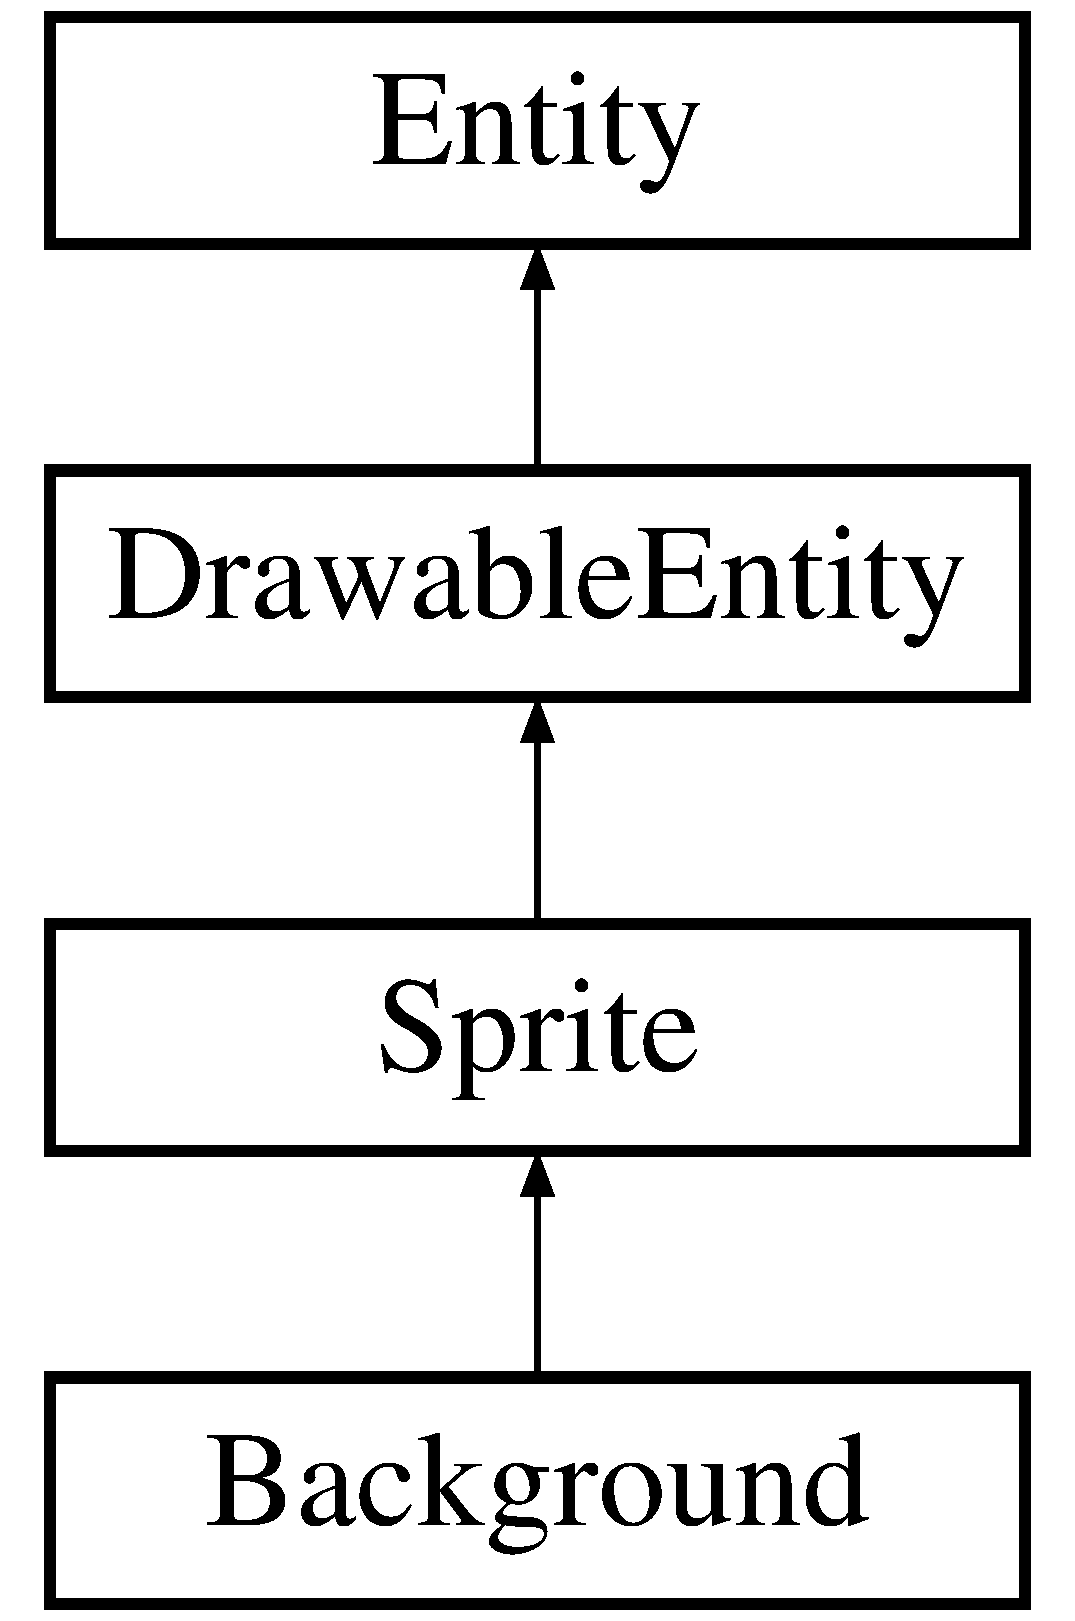
\includegraphics[height=4.000000cm]{class_sprite}
\end{center}
\end{figure}
\subsection*{Public Member Functions}
\begin{DoxyCompactItemize}
\item 
\hyperlink{class_sprite_a8accab430f9d90ae5117b57d67e32b84}{$\sim$\+Sprite} ()
\item 
void \hyperlink{class_sprite_a51cf0234a0f71f4c9fb722a9e331305a}{init} (const float px, const float py, const float rotation, const float scalex, const float scaley, const sf\+::\+Texture \&texture)
\item 
void \hyperlink{class_sprite_af9c2ffd6e4c3f1cc1791562be86fe2cc}{init} (const float px, const float py, const float rotation, const float scalex, const float scaley, const sf\+::\+Texture \&texture, uint8\+\_\+t \&error\+\_\+ocurred)
\item 
uint8\+\_\+t \hyperlink{class_sprite_ae60101c72db08a33215ec89faae8a87c}{init} (const float px, const float py, const float rotation, const float scalex, const float scaley, const std\+::string \&file\+\_\+path)
\item 
void \hyperlink{class_sprite_adf1e840c7fe51abacc8a8f80c9e63c81}{draw} (sf\+::\+Render\+Window \&window)
\item 
bool \hyperlink{class_sprite_acb1a84678f2536ff83b5f2c44dfa3b45}{check\+Collision} (const sf\+::\+Vector2f \&position)
\item 
void \hyperlink{class_sprite_a26019c4dc52face7a098ddace9926863}{unuse} ()
\item 
Sprite\+Origin \hyperlink{class_sprite_a0eccfb75237b7c5eda33810cb1080daf}{origin} ()
\end{DoxyCompactItemize}
\subsection*{Static Public Member Functions}
\begin{DoxyCompactItemize}
\item 
static \hyperlink{class_sprite}{Sprite} $\ast$ \hyperlink{class_sprite_aaabea785dc01ff0246b290fc9e6b3f62}{Create\+Sprite} ()
\end{DoxyCompactItemize}
\subsection*{Public Attributes}
\begin{DoxyCompactItemize}
\item 
\mbox{\Hypertarget{class_sprite_abf366a9a6edad58a8e2bb8a61cc2c3cd}\label{class_sprite_abf366a9a6edad58a8e2bb8a61cc2c3cd}} 
sf\+::\+Sprite {\bfseries sprite\+\_\+}
\item 
\mbox{\Hypertarget{class_sprite_a06bd345188635cf4ecd14c0388458f87}\label{class_sprite_a06bd345188635cf4ecd14c0388458f87}} 
std\+::string {\bfseries texture\+\_\+dir\+\_\+}
\end{DoxyCompactItemize}
\subsection*{Static Public Attributes}
\begin{DoxyCompactItemize}
\item 
\mbox{\Hypertarget{class_sprite_a9f565e1571739b17c22760fa99289d2a}\label{class_sprite_a9f565e1571739b17c22760fa99289d2a}} 
static const uint8\+\_\+t {\bfseries k\+Max\+Sprites} = 50
\end{DoxyCompactItemize}
\subsection*{Protected Member Functions}
\begin{DoxyCompactItemize}
\item 
\hyperlink{class_sprite_a12cba3ac1868418add3c4d95ce87e615}{Sprite} ()
\item 
\hyperlink{class_sprite_aa5cb9fac0cfa5d81dc429e75137179d0}{Sprite} (const \hyperlink{class_sprite}{Sprite} \&o)
\end{DoxyCompactItemize}
\subsection*{Protected Attributes}
\begin{DoxyCompactItemize}
\item 
\mbox{\Hypertarget{class_sprite_adc21e288d7f99213c4b0ef37eaa58353}\label{class_sprite_adc21e288d7f99213c4b0ef37eaa58353}} 
sf\+::\+Texture $\ast$ {\bfseries own\+\_\+texture\+\_\+}
\end{DoxyCompactItemize}
\subsection*{Static Protected Attributes}
\begin{DoxyCompactItemize}
\item 
\mbox{\Hypertarget{class_sprite_a1fc1356f60c3d969a5f4cf6b70759e0e}\label{class_sprite_a1fc1356f60c3d969a5f4cf6b70759e0e}} 
static uint32\+\_\+t {\bfseries total\+\_\+sprites\+\_\+}
\end{DoxyCompactItemize}


\subsection{Detailed Description}
entity \hyperlink{class_sprite}{Sprite}

Class used to represent a sprite. 

\subsection{Constructor \& Destructor Documentation}
\mbox{\Hypertarget{class_sprite_a8accab430f9d90ae5117b57d67e32b84}\label{class_sprite_a8accab430f9d90ae5117b57d67e32b84}} 
\index{Sprite@{Sprite}!````~Sprite@{$\sim$\+Sprite}}
\index{````~Sprite@{$\sim$\+Sprite}!Sprite@{Sprite}}
\subsubsection{\texorpdfstring{$\sim$\+Sprite()}{~Sprite()}}
{\footnotesize\ttfamily Sprite\+::$\sim$\+Sprite (\begin{DoxyParamCaption}{ }\end{DoxyParamCaption})}

a sprite

In case the sprite stored it\textquotesingle{}s own texture in the hip it needs to free it. \mbox{\Hypertarget{class_sprite_a12cba3ac1868418add3c4d95ce87e615}\label{class_sprite_a12cba3ac1868418add3c4d95ce87e615}} 
\index{Sprite@{Sprite}!Sprite@{Sprite}}
\index{Sprite@{Sprite}!Sprite@{Sprite}}
\subsubsection{\texorpdfstring{Sprite()}{Sprite()}\hspace{0.1cm}{\footnotesize\ttfamily [1/2]}}
{\footnotesize\ttfamily Sprite\+::\+Sprite (\begin{DoxyParamCaption}{ }\end{DoxyParamCaption})\hspace{0.3cm}{\ttfamily [protected]}}

constructor

\hyperlink{class_sprite}{Sprite} constructor used by the factory to create sprite

\begin{DoxyReturn}{Returns}
$\ast$\+Sprite 
\end{DoxyReturn}
\mbox{\Hypertarget{class_sprite_aa5cb9fac0cfa5d81dc429e75137179d0}\label{class_sprite_aa5cb9fac0cfa5d81dc429e75137179d0}} 
\index{Sprite@{Sprite}!Sprite@{Sprite}}
\index{Sprite@{Sprite}!Sprite@{Sprite}}
\subsubsection{\texorpdfstring{Sprite()}{Sprite()}\hspace{0.1cm}{\footnotesize\ttfamily [2/2]}}
{\footnotesize\ttfamily Sprite\+::\+Sprite (\begin{DoxyParamCaption}\item[{const \hyperlink{class_sprite}{Sprite} \&}]{o }\end{DoxyParamCaption})\hspace{0.3cm}{\ttfamily [inline]}, {\ttfamily [protected]}}

copy constructor

\hyperlink{class_sprite}{Sprite} copy constructor without anything to disable it.

\begin{DoxyReturn}{Returns}
$\ast$\+Sprite 
\end{DoxyReturn}


\subsection{Member Function Documentation}
\mbox{\Hypertarget{class_sprite_acb1a84678f2536ff83b5f2c44dfa3b45}\label{class_sprite_acb1a84678f2536ff83b5f2c44dfa3b45}} 
\index{Sprite@{Sprite}!check\+Collision@{check\+Collision}}
\index{check\+Collision@{check\+Collision}!Sprite@{Sprite}}
\subsubsection{\texorpdfstring{check\+Collision()}{checkCollision()}}
{\footnotesize\ttfamily bool Sprite\+::check\+Collision (\begin{DoxyParamCaption}\item[{const sf\+::\+Vector2f \&}]{position }\end{DoxyParamCaption})}

if a point collides with the sprite

Checks if the point passed by reference collides with the sprite.

\begin{DoxyReturn}{Returns}
bool returns true if the point collides and false if not. 
\end{DoxyReturn}
\mbox{\Hypertarget{class_sprite_aaabea785dc01ff0246b290fc9e6b3f62}\label{class_sprite_aaabea785dc01ff0246b290fc9e6b3f62}} 
\index{Sprite@{Sprite}!Create\+Sprite@{Create\+Sprite}}
\index{Create\+Sprite@{Create\+Sprite}!Sprite@{Sprite}}
\subsubsection{\texorpdfstring{Create\+Sprite()}{CreateSprite()}}
{\footnotesize\ttfamily static \hyperlink{class_sprite}{Sprite}$\ast$ Sprite\+::\+Create\+Sprite (\begin{DoxyParamCaption}{ }\end{DoxyParamCaption})\hspace{0.3cm}{\ttfamily [static]}}

that creates sprites

Checks that the number of sprites didn\textquotesingle{}t pass the maxim amount established If you wish to create a \hyperlink{class_sprite}{Sprite} you must use this method. In case the maximum amount of sprites has been reached it will return nullptr. Otherwise it will return a pointer to a sprite.

\begin{DoxyReturn}{Returns}
Sprite$\ast$ returns the sprite created or nullptr if the maximum of sprites has been reached 
\end{DoxyReturn}
\mbox{\Hypertarget{class_sprite_adf1e840c7fe51abacc8a8f80c9e63c81}\label{class_sprite_adf1e840c7fe51abacc8a8f80c9e63c81}} 
\index{Sprite@{Sprite}!draw@{draw}}
\index{draw@{draw}!Sprite@{Sprite}}
\subsubsection{\texorpdfstring{draw()}{draw()}}
{\footnotesize\ttfamily void Sprite\+::draw (\begin{DoxyParamCaption}\item[{sf\+::\+Render\+Window \&}]{window }\end{DoxyParamCaption})}

the graphic entity \hyperlink{class_sprite}{Sprite}

Draws the sprite using S\+F\+ML to the window passed by reference

\begin{DoxyReturn}{Returns}
void 
\end{DoxyReturn}

\begin{DoxyParams}{Parameters}
{\em window} & S\+F\+ML Render\+Window passed by reference \\
\hline
\end{DoxyParams}
\mbox{\Hypertarget{class_sprite_a51cf0234a0f71f4c9fb722a9e331305a}\label{class_sprite_a51cf0234a0f71f4c9fb722a9e331305a}} 
\index{Sprite@{Sprite}!init@{init}}
\index{init@{init}!Sprite@{Sprite}}
\subsubsection{\texorpdfstring{init()}{init()}\hspace{0.1cm}{\footnotesize\ttfamily [1/3]}}
{\footnotesize\ttfamily void Sprite\+::init (\begin{DoxyParamCaption}\item[{const float}]{px,  }\item[{const float}]{py,  }\item[{const float}]{rotation,  }\item[{const float}]{scalex,  }\item[{const float}]{scaley,  }\item[{const sf\+::\+Texture \&}]{texture }\end{DoxyParamCaption})}

the sprite using a texture

Initializes the position and transformations of a sprite using an sf\+::\+Texture as texture.

\begin{DoxyReturn}{Returns}
void 
\end{DoxyReturn}

\begin{DoxyParams}{Parameters}
{\em px} & position x of the sprite \\
\hline
{\em py} & position y of the sprite \\
\hline
{\em rotation} & value of rotation of the sprite in degrees \\
\hline
{\em scalex} & x scale value of the sprite \\
\hline
{\em scaley} & y scale value of the sprite \\
\hline
{\em texture} & that will use the sprite \\
\hline
\end{DoxyParams}
\mbox{\Hypertarget{class_sprite_af9c2ffd6e4c3f1cc1791562be86fe2cc}\label{class_sprite_af9c2ffd6e4c3f1cc1791562be86fe2cc}} 
\index{Sprite@{Sprite}!init@{init}}
\index{init@{init}!Sprite@{Sprite}}
\subsubsection{\texorpdfstring{init()}{init()}\hspace{0.1cm}{\footnotesize\ttfamily [2/3]}}
{\footnotesize\ttfamily void Sprite\+::init (\begin{DoxyParamCaption}\item[{const float}]{px,  }\item[{const float}]{py,  }\item[{const float}]{rotation,  }\item[{const float}]{scalex,  }\item[{const float}]{scaley,  }\item[{const sf\+::\+Texture \&}]{texture,  }\item[{uint8\+\_\+t \&}]{error\+\_\+ocurred }\end{DoxyParamCaption})}

the sprite using a buffer from memory

Initializes an \hyperlink{class_sprite}{Sprite} with its own texture that will be stored in memory. In case the allocation of the texture fails it will return a 0. If all went well 1

\begin{DoxyReturn}{Returns}
void 
\end{DoxyReturn}

\begin{DoxyParams}{Parameters}
{\em px} & position x of the sprite \\
\hline
{\em py} & position y of the sprite \\
\hline
{\em rotation} & value of rotation of the sprite in degrees \\
\hline
{\em scalex} & x scale value of the sprite \\
\hline
{\em scaley} & y scale value of the sprite \\
\hline
{\em texture} & referency of the texture we wish to do the copy \\
\hline
{\em error\+\_\+ocurred} & indicates if there was an error in the execution \\
\hline
\end{DoxyParams}
\mbox{\Hypertarget{class_sprite_ae60101c72db08a33215ec89faae8a87c}\label{class_sprite_ae60101c72db08a33215ec89faae8a87c}} 
\index{Sprite@{Sprite}!init@{init}}
\index{init@{init}!Sprite@{Sprite}}
\subsubsection{\texorpdfstring{init()}{init()}\hspace{0.1cm}{\footnotesize\ttfamily [3/3]}}
{\footnotesize\ttfamily uint8\+\_\+t Sprite\+::init (\begin{DoxyParamCaption}\item[{const float}]{px,  }\item[{const float}]{py,  }\item[{const float}]{rotation,  }\item[{const float}]{scalex,  }\item[{const float}]{scaley,  }\item[{const std\+::string \&}]{file\+\_\+path }\end{DoxyParamCaption})}

the sprite using an image file

Initializes an \hyperlink{class_sprite}{Sprite} with its own texture through an image file. In case the allocation of the texture fails it will return a 0. If all went well 1

\begin{DoxyReturn}{Returns}
uint8\+\_\+t indicates if there was an error in the execution error-\/$>$1 ok-\/$>$0 
\end{DoxyReturn}

\begin{DoxyParams}{Parameters}
{\em px} & position x of the sprite \\
\hline
{\em py} & position y of the sprite \\
\hline
{\em rotation} & value of rotation of the sprite in degrees \\
\hline
{\em scalex} & x scale value of the sprite \\
\hline
{\em scaley} & y scale value of the sprite \\
\hline
{\em file\+\_\+path} & image that will be used for the texture \\
\hline
\end{DoxyParams}
\mbox{\Hypertarget{class_sprite_a0eccfb75237b7c5eda33810cb1080daf}\label{class_sprite_a0eccfb75237b7c5eda33810cb1080daf}} 
\index{Sprite@{Sprite}!origin@{origin}}
\index{origin@{origin}!Sprite@{Sprite}}
\subsubsection{\texorpdfstring{origin()}{origin()}}
{\footnotesize\ttfamily Sprite\+Origin Sprite\+::origin (\begin{DoxyParamCaption}{ }\end{DoxyParamCaption})}

for origin Returns the origin of the texture, it will vary depending on how the sprite was initiallized

\begin{DoxyReturn}{Returns}
void 
\end{DoxyReturn}
\mbox{\Hypertarget{class_sprite_a26019c4dc52face7a098ddace9926863}\label{class_sprite_a26019c4dc52face7a098ddace9926863}} 
\index{Sprite@{Sprite}!unuse@{unuse}}
\index{unuse@{unuse}!Sprite@{Sprite}}
\subsubsection{\texorpdfstring{unuse()}{unuse()}}
{\footnotesize\ttfamily void Sprite\+::unuse (\begin{DoxyParamCaption}{ }\end{DoxyParamCaption})}

the values of the sprite

Sets the attributes of the sprite to a default value to return it to a pool and being able to reuse it later.

\begin{DoxyReturn}{Returns}
void 
\end{DoxyReturn}


The documentation for this class was generated from the following file\+:\begin{DoxyCompactItemize}
\item 
include/sprite.\+h\end{DoxyCompactItemize}

\hypertarget{class_window}{}\section{Window Class Reference}
\label{class_window}\index{Window@{Window}}


{\ttfamily \#include $<$window.\+h$>$}

\subsection*{Public Member Functions}
\begin{DoxyCompactItemize}
\item 
bool \hyperlink{class_window_a0530ead23b2c91ef90a5f98e4df41cb8}{is\+Open} ()
\begin{DoxyCompactList}\small\item\em Checks if the window is open. \end{DoxyCompactList}\item 
void \hyperlink{class_window_afadfafa5a0b9472554759004aafb327e}{display} ()
\begin{DoxyCompactList}\small\item\em Display the window. \end{DoxyCompactList}\item 
void \hyperlink{class_window_a35055c04498121d39741bfcd5082705b}{close} ()
\begin{DoxyCompactList}\small\item\em Close the window. \end{DoxyCompactList}\item 
void \hyperlink{class_window_a38bc43bdd1a97e5de7f346ba4c3957ef}{clear} ()
\begin{DoxyCompactList}\small\item\em Clear the window. \end{DoxyCompactList}\item 
void \hyperlink{class_window_adfb2d5826942693e289d13f314a341f7}{draw} (const sf\+::\+Drawable \&drawable)
\begin{DoxyCompactList}\small\item\em Draw a drawable object. \end{DoxyCompactList}\end{DoxyCompactItemize}
\subsection*{Static Public Member Functions}
\begin{DoxyCompactItemize}
\item 
static \hyperlink{class_window}{Window} $\ast$ \hyperlink{class_window_ac23ace79f02693ff5463f91dba8bb38b}{Create\+Window} (const sf\+::\+Vector2u size, const sf\+::\+String \&title, unsigned int frame\+Rate\+Limit=60)
\begin{DoxyCompactList}\small\item\em Factory that creates windows. \end{DoxyCompactList}\end{DoxyCompactItemize}
\subsection*{Public Attributes}
\begin{DoxyCompactItemize}
\item 
\mbox{\Hypertarget{class_window_adf4fd93b0ad5bd9c045a4bbc5c767b7d}\label{class_window_adf4fd93b0ad5bd9c045a4bbc5c767b7d}} 
unsigned int {\bfseries frame\+\_\+rate\+\_\+limit\+\_\+}
\item 
\mbox{\Hypertarget{class_window_a49d4bbd674a3cef9ff823ef17a0bef42}\label{class_window_a49d4bbd674a3cef9ff823ef17a0bef42}} 
sf\+::\+Render\+Window $\ast$ {\bfseries sfml\+\_\+window\+\_\+}
\item 
\mbox{\Hypertarget{class_window_a79a1f398d58121ef49bb7d29b3f2ea64}\label{class_window_a79a1f398d58121ef49bb7d29b3f2ea64}} 
sf\+::\+Event {\bfseries event\+\_\+}
\end{DoxyCompactItemize}
\subsection*{Static Public Attributes}
\begin{DoxyCompactItemize}
\item 
\mbox{\Hypertarget{class_window_adddb1eb449be45c372249dc1462c4e68}\label{class_window_adddb1eb449be45c372249dc1462c4e68}} 
static const uint8\+\_\+t {\bfseries k\+Max\+Windows} = 1
\end{DoxyCompactItemize}


\subsection{Detailed Description}
Class create and manage the windows

This class create and manage the windows of the game editor 

\subsection{Member Function Documentation}
\mbox{\Hypertarget{class_window_a38bc43bdd1a97e5de7f346ba4c3957ef}\label{class_window_a38bc43bdd1a97e5de7f346ba4c3957ef}} 
\index{Window@{Window}!clear@{clear}}
\index{clear@{clear}!Window@{Window}}
\subsubsection{\texorpdfstring{clear()}{clear()}}
{\footnotesize\ttfamily void Window\+::clear (\begin{DoxyParamCaption}{ }\end{DoxyParamCaption})}



Clear the window. 

Clear the window and put it black.

\begin{DoxyReturn}{Returns}
void. 
\end{DoxyReturn}
\mbox{\Hypertarget{class_window_a35055c04498121d39741bfcd5082705b}\label{class_window_a35055c04498121d39741bfcd5082705b}} 
\index{Window@{Window}!close@{close}}
\index{close@{close}!Window@{Window}}
\subsubsection{\texorpdfstring{close()}{close()}}
{\footnotesize\ttfamily void Window\+::close (\begin{DoxyParamCaption}{ }\end{DoxyParamCaption})}



Close the window. 

Close the window.

\begin{DoxyReturn}{Returns}
void. 
\end{DoxyReturn}
\mbox{\Hypertarget{class_window_ac23ace79f02693ff5463f91dba8bb38b}\label{class_window_ac23ace79f02693ff5463f91dba8bb38b}} 
\index{Window@{Window}!Create\+Window@{Create\+Window}}
\index{Create\+Window@{Create\+Window}!Window@{Window}}
\subsubsection{\texorpdfstring{Create\+Window()}{CreateWindow()}}
{\footnotesize\ttfamily static \hyperlink{class_window}{Window}$\ast$ Window\+::\+Create\+Window (\begin{DoxyParamCaption}\item[{const sf\+::\+Vector2u}]{size,  }\item[{const sf\+::\+String \&}]{title,  }\item[{unsigned int}]{frame\+Rate\+Limit = {\ttfamily 60} }\end{DoxyParamCaption})\hspace{0.3cm}{\ttfamily [static]}}



Factory that creates windows. 

Checks that the number of window didn\textquotesingle{}t pass the maxim established. In case the maximum of window has been reached it will return nullptr.

\begin{DoxyReturn}{Returns}
Window$\ast$ returns a pointer to the \hyperlink{class_window}{Window} created or nullptr if the maximum of windows has been reached 
\end{DoxyReturn}
\mbox{\Hypertarget{class_window_afadfafa5a0b9472554759004aafb327e}\label{class_window_afadfafa5a0b9472554759004aafb327e}} 
\index{Window@{Window}!display@{display}}
\index{display@{display}!Window@{Window}}
\subsubsection{\texorpdfstring{display()}{display()}}
{\footnotesize\ttfamily void Window\+::display (\begin{DoxyParamCaption}{ }\end{DoxyParamCaption})}



Display the window. 

Display on screen the elements that has been rendered to the window so far.

\begin{DoxyReturn}{Returns}
void. 
\end{DoxyReturn}
\mbox{\Hypertarget{class_window_adfb2d5826942693e289d13f314a341f7}\label{class_window_adfb2d5826942693e289d13f314a341f7}} 
\index{Window@{Window}!draw@{draw}}
\index{draw@{draw}!Window@{Window}}
\subsubsection{\texorpdfstring{draw()}{draw()}}
{\footnotesize\ttfamily void Window\+::draw (\begin{DoxyParamCaption}\item[{const sf\+::\+Drawable \&}]{drawable }\end{DoxyParamCaption})}



Draw a drawable object. 

Draw a drawable object to the render-\/target.

\begin{DoxyReturn}{Returns}
void. 
\end{DoxyReturn}
\mbox{\Hypertarget{class_window_a0530ead23b2c91ef90a5f98e4df41cb8}\label{class_window_a0530ead23b2c91ef90a5f98e4df41cb8}} 
\index{Window@{Window}!is\+Open@{is\+Open}}
\index{is\+Open@{is\+Open}!Window@{Window}}
\subsubsection{\texorpdfstring{is\+Open()}{isOpen()}}
{\footnotesize\ttfamily bool Window\+::is\+Open (\begin{DoxyParamCaption}{ }\end{DoxyParamCaption})}



Checks if the window is open. 

Checks if the window is open.

\begin{DoxyReturn}{Returns}
bool returns true if the window is open and false if not. 
\end{DoxyReturn}


The documentation for this class was generated from the following file\+:\begin{DoxyCompactItemize}
\item 
C\+:/\+E\+S\+A\+T/2pa\+\_\+ma\+\_\+martinezcajm/2d\+\_\+engine/include/window.\+h\end{DoxyCompactItemize}

%--- End generated contents ---

% Index
\backmatter
\newpage
\phantomsection
\clearemptydoublepage
\addcontentsline{toc}{chapter}{Index}
\printindex

\end{document}
